% Options for packages loaded elsewhere
\PassOptionsToPackage{unicode}{hyperref}
\PassOptionsToPackage{hyphens}{url}
\PassOptionsToPackage{dvipsnames,svgnames,x11names}{xcolor}
%
\documentclass[
]{article}

\usepackage{amsmath,amssymb}
\usepackage{iftex}
\ifPDFTeX
  \usepackage[T1]{fontenc}
  \usepackage[utf8]{inputenc}
  \usepackage{textcomp} % provide euro and other symbols
\else % if luatex or xetex
  \usepackage{unicode-math}
  \defaultfontfeatures{Scale=MatchLowercase}
  \defaultfontfeatures[\rmfamily]{Ligatures=TeX,Scale=1}
\fi
\usepackage{lmodern}
\ifPDFTeX\else  
    % xetex/luatex font selection
\fi
% Use upquote if available, for straight quotes in verbatim environments
\IfFileExists{upquote.sty}{\usepackage{upquote}}{}
\IfFileExists{microtype.sty}{% use microtype if available
  \usepackage[]{microtype}
  \UseMicrotypeSet[protrusion]{basicmath} % disable protrusion for tt fonts
}{}
\makeatletter
\@ifundefined{KOMAClassName}{% if non-KOMA class
  \IfFileExists{parskip.sty}{%
    \usepackage{parskip}
  }{% else
    \setlength{\parindent}{0pt}
    \setlength{\parskip}{6pt plus 2pt minus 1pt}}
}{% if KOMA class
  \KOMAoptions{parskip=half}}
\makeatother
\usepackage{xcolor}
\setlength{\emergencystretch}{3em} % prevent overfull lines
\setcounter{secnumdepth}{-\maxdimen} % remove section numbering
% Make \paragraph and \subparagraph free-standing
\ifx\paragraph\undefined\else
  \let\oldparagraph\paragraph
  \renewcommand{\paragraph}[1]{\oldparagraph{#1}\mbox{}}
\fi
\ifx\subparagraph\undefined\else
  \let\oldsubparagraph\subparagraph
  \renewcommand{\subparagraph}[1]{\oldsubparagraph{#1}\mbox{}}
\fi


\providecommand{\tightlist}{%
  \setlength{\itemsep}{0pt}\setlength{\parskip}{0pt}}\usepackage{longtable,booktabs,array}
\usepackage{calc} % for calculating minipage widths
% Correct order of tables after \paragraph or \subparagraph
\usepackage{etoolbox}
\makeatletter
\patchcmd\longtable{\par}{\if@noskipsec\mbox{}\fi\par}{}{}
\makeatother
% Allow footnotes in longtable head/foot
\IfFileExists{footnotehyper.sty}{\usepackage{footnotehyper}}{\usepackage{footnote}}
\makesavenoteenv{longtable}
\usepackage{graphicx}
\makeatletter
\def\maxwidth{\ifdim\Gin@nat@width>\linewidth\linewidth\else\Gin@nat@width\fi}
\def\maxheight{\ifdim\Gin@nat@height>\textheight\textheight\else\Gin@nat@height\fi}
\makeatother
% Scale images if necessary, so that they will not overflow the page
% margins by default, and it is still possible to overwrite the defaults
% using explicit options in \includegraphics[width, height, ...]{}
\setkeys{Gin}{width=\maxwidth,height=\maxheight,keepaspectratio}
% Set default figure placement to htbp
\makeatletter
\def\fps@figure{htbp}
\makeatother
% definitions for citeproc citations
\NewDocumentCommand\citeproctext{}{}
\NewDocumentCommand\citeproc{mm}{%
  \begingroup\def\citeproctext{#2}\cite{#1}\endgroup}
\makeatletter
 % allow citations to break across lines
 \let\@cite@ofmt\@firstofone
 % avoid brackets around text for \cite:
 \def\@biblabel#1{}
 \def\@cite#1#2{{#1\if@tempswa , #2\fi}}
\makeatother
\newlength{\cslhangindent}
\setlength{\cslhangindent}{1.5em}
\newlength{\csllabelwidth}
\setlength{\csllabelwidth}{3em}
\newenvironment{CSLReferences}[2] % #1 hanging-indent, #2 entry-spacing
 {\begin{list}{}{%
  \setlength{\itemindent}{0pt}
  \setlength{\leftmargin}{0pt}
  \setlength{\parsep}{0pt}
  % turn on hanging indent if param 1 is 1
  \ifodd #1
   \setlength{\leftmargin}{\cslhangindent}
   \setlength{\itemindent}{-1\cslhangindent}
  \fi
  % set entry spacing
  \setlength{\itemsep}{#2\baselineskip}}}
 {\end{list}}
\usepackage{calc}
\newcommand{\CSLBlock}[1]{\hfill\break\parbox[t]{\linewidth}{\strut\ignorespaces#1\strut}}
\newcommand{\CSLLeftMargin}[1]{\parbox[t]{\csllabelwidth}{\strut#1\strut}}
\newcommand{\CSLRightInline}[1]{\parbox[t]{\linewidth - \csllabelwidth}{\strut#1\strut}}
\newcommand{\CSLIndent}[1]{\hspace{\cslhangindent}#1}

\usepackage{booktabs}
\usepackage{caption}
\usepackage{longtable}
\usepackage{colortbl}
\usepackage{array}
\usepackage{anyfontsize}
\usepackage{multirow}
\usepackage{draftwatermark}
\SetWatermarkText{DRAFT}
\SetWatermarkScale{1.5}
\SetWatermarkColor[gray]{0.95}
\usepackage{float}
\floatplacement{table}{H}
\floatplacement{figure}{H}
\makeatletter
\@ifpackageloaded{caption}{}{\usepackage{caption}}
\AtBeginDocument{%
\ifdefined\contentsname
  \renewcommand*\contentsname{Table of contents}
\else
  \newcommand\contentsname{Table of contents}
\fi
\ifdefined\listfigurename
  \renewcommand*\listfigurename{List of Figures}
\else
  \newcommand\listfigurename{List of Figures}
\fi
\ifdefined\listtablename
  \renewcommand*\listtablename{List of Tables}
\else
  \newcommand\listtablename{List of Tables}
\fi
\ifdefined\figurename
  \renewcommand*\figurename{Figure}
\else
  \newcommand\figurename{Figure}
\fi
\ifdefined\tablename
  \renewcommand*\tablename{Table}
\else
  \newcommand\tablename{Table}
\fi
}
\@ifpackageloaded{float}{}{\usepackage{float}}
\floatstyle{ruled}
\@ifundefined{c@chapter}{\newfloat{codelisting}{h}{lop}}{\newfloat{codelisting}{h}{lop}[chapter]}
\floatname{codelisting}{Listing}
\newcommand*\listoflistings{\listof{codelisting}{List of Listings}}
\makeatother
\makeatletter
\makeatother
\makeatletter
\@ifpackageloaded{caption}{}{\usepackage{caption}}
\@ifpackageloaded{subcaption}{}{\usepackage{subcaption}}
\makeatother
\ifLuaTeX
  \usepackage{selnolig}  % disable illegal ligatures
\fi
\usepackage{bookmark}

\IfFileExists{xurl.sty}{\usepackage{xurl}}{} % add URL line breaks if available
\urlstyle{same} % disable monospaced font for URLs
\hypersetup{
  pdftitle={A family of accessibility measures derived from spatial interaction principles},
  pdfauthor={Anastasia Soukhov; Rafael H. M. Pereira; Christopher D. Higgins; Antonio Páez},
  pdfkeywords={accessibility; spatial interaction model; balancing
factors; competitive accessibility; constraints; singly constrained;
doubly constrained; total constrained},
  colorlinks=true,
  linkcolor={blue},
  filecolor={Maroon},
  citecolor={Blue},
  urlcolor={Blue},
  pdfcreator={LaTeX via pandoc}}

\title{A family of accessibility measures derived from spatial
interaction principles}
\usepackage{etoolbox}
\makeatletter
\providecommand{\subtitle}[1]{% add subtitle to \maketitle
  \apptocmd{\@title}{\par {\large #1 \par}}{}{}
}
\makeatother
\subtitle{Submitted preprint for peer-review (May 2025)}
\author{Anastasia Soukhov \and Rafael H. M. Pereira \and Christopher D.
Higgins \and Antonio Páez}
\date{}

\begin{document}
\maketitle
\begin{abstract}
Transportation planning has long prioritized the efficiency of movement,
or mobility. However, the concept of accessibility represents a more
comprehensive evolution, shifting focus from mere movement to the
potential to reach (i.e., spatially interact) with desired destinations.
Despite growing recognition of accessibility-based planning approaches,
the concept remains fragmented, with inconsistent definitions and
unclear interpretations. This work's aim is to clarify and unify the
concept of accessibility by connecting it into spatial interaction
modeling. We demonstrate that widely used mobility and accessibility
models, such as gravity-based accessibility and spatial interaction
models, share common theoretical roots. From this foundation, this paper
offers three contributions: (A) we introduce a family of accessibility
measures within the principles of spatial interaction, and (B) formally
define four members of the family, namely the `unconstrained' measure
(i.e., Hansen-type accessibility), the `total constrained' measure
(i.e., a constrained version of the Hansen-type accessibility), the
`singly constrained' measure (i.e., related to the popular two step
floating catchment approach - 2SFCA), and the `doubly constrained'
measure representing realized interactions or `access', effectively
equal to the doubly constrained spatial interaction model; and (C) we
demonstrate the interpretability advantages of the family, as these
constrained accessibility measures yield values in units of the number
of potential ``opportunities for spatial interaction'' or ``population
for spatial interaction'' for each zone and zonal flow. The family of
accessibility measures proposed here clarifies the concept of
`potential' in accessibility, demonstrates theoretical and formulaic
linkages across popular accessibility and spatial interaction models,
and reintroduces measurement units into accessibility measures. By doing
so, we believe this family of measures can unlock a clearer, more
interpretable, and cohesive foundation for accessibility analysis.
\end{abstract}

\section{Introduction}\label{introduction}

In the early nineteenth century, industrializing cities grew rapidly: so
did traffic congestion and the development of transportation planning
practice focused primarily on mobility. In this newly founded practice,
access to destinations was treated as a by-product of movement.
Following the rise of the automobile and significant investments in
transportation infrastructure after World War II, this mobility-oriented
approach has led to some problematic outcomes. Specifically, the car
became seen as the ultimate mobility tool, helping to foster the
development of low-density, single-use residential neighborhoods and
entrenching an automobility mono-culture within transportation systems
(H. J. Miller 2011; Lavery, Páez, and Kanaroglou 2013). Decades of
planning for this automobility mono-culture, still often characterized
by road and highway expansion, have been marked by increased travel
costs and environmental burdens, with limited impact on enhancing the
ease with which people can reach destinations (Steven Farber and Páez
2011; S. Handy 2002; Páez et al. 2010). In response, transportation
researchers have increasingly advocated for the adoption of
accessibility as a planning criterion, in contrast to traditional
mobility-oriented transportation planning approaches which translate
into indicators that benchmark movement (e.g., vehicle kilometres
traveled, intersection through traffic, etc.) which are not necessarily
linked to improved accessibility (Silva et al. 2017; Paez et al. 2013;
S. Handy 2020; El-Geneidy and Levinson 2022).

Accessibility may be defined as the ``potential of opportunities for
{[}spatial{]} interaction'' (Hansen 1959), in contrast to mobility which
is simply, movement in itself or `spatial interaction'. Mobility has
been the basis of traditional transportation planning approaches
(Ortúzar and Willumsen 2011). While accessibility brings a more holistic
understanding of combined transportation and land use systems,
incorporating both the explicit consideration of destination as
opportunity and the concept of \emph{potential} (S. L. Handy and
Niemeier 1997).

The growing interest in accessibility has been accompanied by a boom in
scholarly research using different methods and focusing on different
research contexts; it has grown to include studies of access to
employment (e.g., Karst and Van Eck 2003; Grengs 2010; Páez et al. 2013;
Merlin and Hu 2017; Tao et al. 2020), health care (e.g., Luo and Wang
2003; Páez et al. 2010; Wan, Zou, and Sternberg 2012; Delamater 2013;
Boisjoly, Moreno-Monroy, and El-Geneidy 2017; Pereira et al. 2021),
green spaces (Reyes, Paez, and Morency 2014; Rojas et al. 2016; Liang,
Yan, and Yan 2024), schools (e.g., Williams and Wang 2014; Romanillos
and Garcia-Palomares 2018; Marques, Wolf, and Feitosa 2021), social
contacts (e.g., Neutens et al. 2007; S. Farber, Páez, and Morency 2012;
S. Farber et al. 2013), and regional economic analysis (e.g., R.
Vickerman, Spiekermann, and Wegener 1999; Lopez, Gutierrez, and Gomez
2008; Ribeiro, Antunes, and Páez 2010; Gutierrez et al. 2011) among many
other domains of application. In other words, accessibility analysis is
used today to broadly understand the potential to reach (or spatially
interact with) opportunities that are important to people (Ferreira and
Papa 2020). However, despite its growth in popularity in scholarly
works, challenges remain with respect to the more widespread adoption of
accessibility in planning practice. For instance, the diversity of
accessibility definitions has been flagged by van Wee (2016), S. Handy
(2020), and Kapatsila et al. (2023). Further, difficulties in the
interpretability and communicability of outputs has also been noticed by
many authores, including Karst T. Geurs and van Wee (2004), van Wee
(2016), and Ferreira and Papa (2020).

The adoption of accessibility in planning practice is not necessarily
made easier when potential adopters have to contend with a plethora of
definitions, each seemingly more sophisticated but less intuitive than
the last (Kapatsila et al. 2023). At a high level, Karst T. Geurs and
van Wee (2004) identify four families of accessibility measures:
infrastructure-, place-, person-, and utility-based. Of the place-based
family, which is the focus of this paper, the menu has grown to include
gravity-based accessibility (e.g., Hansen 1959; Pirie 1979), cumulative
opportunities (e.g., Wachs and Kumagai 1973; Pirie 1979; Ye et al.
2018), modified gravity (e.g., Schuurman, Berube, and Crooks 2010),
2-Step Floating Catchment Areas (e.g., Luo and Wang 2003), Enhanced
2-Step Floating Catchment Areas (e.g., Luo and Qi 2009), 3-Stage
Floating Catchment Areas (e.g., Wan, Zou, and Sternberg 2012), Modified
2-Step Floating Catchment Areas (e.g., Delamater 2013), inverse 2-Step
Floating Catchment Areas (e.g., F. Wang 2021), and n-steps Floating
Catchment Areas (Liang, Yan, and Yan 2024). How is a practitioner to
choose among this myriad options? What differences in accessibility
scores should matter, and how should they be communicated? {[}see van
Wee (2016); p.~14{]}.

Here, we seek to address the breath of place-based accessibility's
definitions and lack of interpretability by demonstrating that
mobility-oriented models--such as the commonly used gravity-based
accessibility (e.g., Hansen 1959) and the spatial interaction model
(e.g., Wilson 1971)-- are rooted in the same spatial interaction
modeling foundation. In fact, we propose that accessibility can be
specified using spatial interaction principles as a \emph{family of
measures}, akin to the family of spatial interaction models introduced
in Wilson (1971) that can be defined using balancing factors that
constrains values based on known information about the land-use.

This work aims to offer three contributions: (1) it introduces a family
of accessibility measures within the principles of spatial interaction;
(2) it formally defines three \emph{constrained} accessibility measures
by reintroducing Wilson-analogous balancing factors. These measures are
the total constrained accessibility measure, the singly constrained
accessibility measure, and the doubly constrained measure, which are
explicitly connected to popular measures such as the Hansen-type
accessibility (Hansen 1959), the popular competition approach of the
2-Step Floating Catchment Area (2SFCA) (Q. Shen 1998a; Luo and Wang
2003), and the concept of market potential (C. D. Harris 1954; R. W.
Vickerman 1974). These Wilson-analogous balancing factors introduced are
also defined in order of increasing restrictiveness to shed light on the
role of \emph{potential} in accessibility and access. (3) This work also
demonstrates that the introduction of balancing factors makes
accessibility measures easier to interpret and to communicate by
restoring the measurement units to the resulting raw accessibility
values. Each zonal and zonal flow value from a constrained accessibility
measure is always in interpretable units, namely the number of
`opportunities for spatial interaction' or `population for spatial
interaction'. This is in contrast to conventional accessibility
measures, particularly gravity based measures, that yield values in
units of `opportunities weighted by some representation of travel
friction'.

To achieve these stated objectives, this paper contends that
accessibility research must reconnect with its spatial interaction
origins. Particularly, we argue that an important aspect of spatial
interaction modelling--namely, constraining the results to match
empirical observations--was never effectively reincorporated into
accessibility analysis. Empirical constraints were embraced by early
spatial interaction literature following the work of Wilson (1971), but
this stream of literature tended to flow separately from research
inspired by Hansen (1959)' accessibility. The application of Wilson
(1971)`s empirical constraints supported the development of various
spatial interaction models that remain relevant in research and practice
today (Ortúzar and Willumsen 2011). However, the same cannot be said of
the contemporary accessibility literature, where empirical constraints
were not explicitly adopted. We argue that the absence of empirical
constraints (and their attendant proportionality constants) has
contributed to some of accessibility analysis' interpretability issues;
for instance, the fuzziness of insights beyond simple proportional
statements like `higher-than' or `lower-than' (E. J. Miller 2018).
Moreover, without constraints we lose track of what accessibility
measures, that is, the number of opportunities that can be spatially
interacted with. Without a clear sense of measurement units,
comparability between accessibility measures, across cities, and
transport modes, may also become compromised.

Fortunately, accessibility and spatial interaction modelling literature
share common headwaters, and the latter has given careful attention to
measurement units and their interpretability. It is by looking to the
past that we believe accessibility analysis can newly wade into the
future. We continue this work in the following section by tracing the
development of accessibility from its origins in spatial interaction:
from the Newtonian gravitational expression in Ravenstein (1889) through
to the seminal accessibility work of Hansen (1959). We then present
evidence for a narrative highlighting the marked divergence between
accessibility and spatial interaction modelling research after the work
of Wilson (1971). Next, we hark back to Wilson (1971)'s spatial
interaction models, and use them to derive a family of accessibility
measures based on analogous constraints. We illustrate members of this
family of constrained accessibility measures with a simple numerical
example. We then conclude by discussing the uses of these measure and
their interpretation.

\section{Newtonian's roots of human spatial interaction
research}\label{newtonians-roots-of-human-spatial-interaction-research}

The patterns of people's movement in space have been a subject of
scientific inquiry for at least a century and a half. From as far back
as Henry C. Carey's \emph{Principles of Social Science} (Carey 1858), a
concern with the scientific study of human spatial interaction can be
observed. It was in this work where Carey stated that ``man {[}is{]} the
molecule of society {[}and their interaction is subject to{]} the direct
ratio of the mass and the inverse one of distance'' (McKean 1883,
37--38). This statement shows how investigations into human spatial
interaction have often been explicitly coloured by the features of
Newton's Law of Universal Gravitation, first posited in 1687's
\emph{Principia Mathematica} and expressed as in
Equation~\ref{eq-phys-grav-prop}.

\begin{equation}\phantomsection\label{eq-phys-grav-prop}{
F_{ij} \propto \frac{M_i M_j} {D_{ij}^{2}}
}\end{equation}

To be certain, the expression above is one of proportionality, and is
also the most famous in all of science. It states that the force of
attraction \(F\) between a pair of bodies \(i\) and \(j\) is directly
\emph{proportional} to the product of their masses \(M_i\) and \(M_j\),
and inversely \emph{proportional} to the square of the distance between
them \(D_{ij}\). Direct proportionality means that as the product of the
masses increases, so does the force. Likewise, inverse proportionality
means that as the distance increases, the force decreases.
Equation~\ref{eq-phys-grav-prop}, however, does not quantify the
magnitude of the force. To do so, an empirical constant, a.k.a. the
gravitational constant, is required to convert the proportionality into
an equality, ensuring that values of the force \(F\) in
Equation~\ref{eq-phys-grav-prop} match the observed force of attraction
between masses. In other words, Equation~\ref{eq-phys-grav-prop} needs
to be \emph{constrained} using empirical data. Ultimately, the equation
for the force is as seen in Equation~\ref{eq-phys-grav}, where \(G\) is
an empirically calibrated proportionality constant:

\begin{equation}\phantomsection\label{eq-phys-grav}{
F_{ij} = G \frac{M_i M_j} {D_{ij}^{2}}
}\end{equation}

Newton's initial estimate of \(G\) was based on a speculation that the
mean density of earth was between five or six times that of water, an
assumption that received support after Hutton's experiments of 1778
(Hutton 1778, 783). Still, it took over a century from the publication
of \emph{Principia} to refine the estimate of the proportionality
constant to within 1\% accuracy, with Cavendish's 1798 experiment
(Cavendish 1798).

\section{Early research on human spatial interaction: from Ravenstein
(1889) to Stewart
(1948)}\label{early-research-on-human-spatial-interaction-from-ravenstein-1889-to-stewart-1948}

Since the 1880s to the 1940s, a number of researchers theoretically and
empirically attempted to characterise human spatial interaction as some
force of attraction \(F\) that is directly proportion to the masses
\(M_i\) and \(M_j\) and inversely proportional by their separation
distance. This concept was captured with different expressions, but all
tie back to the same Newtonian gravity analogy, although not all of them
included a proportionality constant in their formulation.

Following Carey's \emph{Principles} of 1858, research into human spatial
interaction continued in different contexts. In the late 1880s,
Ravenstein proposed some ``Laws of Migration'' based on his empirical
analysis of migration flows in various countries (Ravenstein 1885,
1889). In these works, Ravenstein posited 1) a directly proportional
relationship between migration flows and the size of destinations (i.e.,
centres of commerce and industry), and 2) an inversely proportional
relationship between the size of flows and the separation between
origins and destinations. As with Carey, these propositions echo
Newton's gravitational laws. Over time, other researchers discovered
similar relationships. For example, Reilly (1929) formulated a law of
retail gravitation, expressed in terms of equal attraction to competing
retail destinations that could be understood as `potential trade
territories'. Later, Zipf proposed a \(\frac{P_1P_2}{D}\) hypothesis for
the case of information (Zipf 1946a), intercity personal movement (Zipf
1946b), and goods movement by railways (Zipf 1946c). The
\(\frac{P_1P_2}{D}\) hypothesis stated that the magnitude of flows was
proportional to the product of the populations of settlements, and
inversely proportional to the distance between them.

A common feature of these early investigations of human spatial
interaction is that a proportionality constant similar to \(G\) in
Equation~\ref{eq-phys-grav} was never considered. Of the researchers
cited above, only Reilly and Zipf expressed their hypotheses in
mathematical terms. Reilly's hypothesis was presented in the following
form:

\begin{equation}\phantomsection\label{eq-reilly}{
B_a = \frac{(P_a\cdot P_T)^N}{D_{aT}^n}
}\end{equation}

\noindent where \(B_a\) is the amount of business drawn to \(a\) from
\(T\), \(P_a\) and \(P_T\) are the populations of the two settlements,
and \(D_{aT}\) is the distance between them. Quantity \(N\) was chosen
by Reilly in a somewhat \emph{ad hoc} fashion as 1, and he used
empirical observations of shoppers to choose a value of \(n = 2\).

Zipf, on the other hand, wrote his hypothesis in mathematical form as:

\begin{equation}\phantomsection\label{eq-zipf}{
C^2 = \frac{P_1\cdot P_2}{D_{12}}
}\end{equation}

\noindent where \(C\) is the volume of goods exchanged between \(1\) and
\(2\), \(P_1\) and \(P_2\) are the populations of the two settlements,
and \(D_{12}\) is the distance between them.

After Carey, it is in Stewart's work on the principles of demographic
gravitation that we find the strongest connection yet to Newton's law
(Stewart 1948). This may relate to academic backgrounds; where Stewart
was a physicist while Ravenstein, Reilly, and Zipf were social
scientists. Besides awareness of preceding research (he cites both
Reilly and Zipf as predecessors in the analysis of human spatial
interaction), Stewart appears to have been the first author to express
his theorized relationships for human spatial interaction with a
proportionality constant \(G\), as follows:

\begin{equation}\phantomsection\label{eq-stewart-force}{
F = G\frac{(\mu_1N_1)(\mu_2N_2)}{d_{12}^2} = G\frac{M_1\cdot M_2}{d_{12}^2} 
}\end{equation}

\noindent Where:

\begin{itemize}
\tightlist
\item
  \(F\) is the \emph{demographic force}
\item
  \(N_1\) and \(N_2\) are the numbers of people of in groups 1 and 2
\item
  \(\mu_1\) and \(\mu_2\) are so-called \emph{molecular weights}, the
  attractive weight of groups 1 and 2
\item
  \(M_1 = \mu_1N_1\) and \(M_2 = \mu_2N_2\) are the demographic masses
  at 1 and 2
\item
  \(d_{12}^2\) is the distance between \(1\) and \(2\)
\item
  And finally \(G\), a constant that Stewart ``left for future
  determination'' (1948, 34)
\end{itemize}

In addition to demographic force, Stewart defined a measure of the
``population potential'' of group \(2\) with respect to group \(1\). In
other words, the potential number of people from location \(2\) that
could visit location \(1\), as follows:

\begin{equation}\phantomsection\label{eq-stewart-population-potential}{
V_1 = G\frac{M_2}{d_{12}}
}\end{equation}

For a system with more than two population bodies, Stewart formulated
the population potential at \(i\) as follows (after arbitrarily assuming
that \(G=1\)):

\begin{equation}\phantomsection\label{eq-stewart-population-potential-integral}{
V_i = \int\frac{D}{r} ds
}\end{equation}

\noindent where \(D\) is the population density over an infinitesimal
area \(ds\) and \(r\) is the distance to \(i\). In
Equation~\ref{eq-stewart-population-potential-integral}, \(D\cdot ds\)
gives an infinitesimal count of the population, say \(dm\), and so,
after discretizing space,
Equation~\ref{eq-stewart-population-potential-integral} can be rewritten
as:

\begin{equation}\phantomsection\label{eq-stewart-population-potential-sum}{
V_i = \sum_j M_jd_{ij}^{-1}
}\end{equation}

Alerted readers will notice that
Equation~\ref{eq-stewart-population-potential-sum}, with some
re-organization of terms, is formally equivalent to our modern
definition of accessibility popularized by Hansen (1959) in the late
1950s.

Stewart's formulation of demographic force, developed in the context of
what he called ``social physics'' (Stewart 1947), was problematic. It
had issues with inconsistent mathematical notation. More seriously
though, Stewart's work was permeated by a view of humans as particles
following physical laws, but tinted by unscientific and racist ideas.
For instance, he assumed that the molecular weight \(\mu\) of the
average American was one, but ``presumably\ldots much less than
one\ldots.for an Australian aborigine'' {[}p.~35{]}. Stewart's ideas
about ``social physics'' soon fell out of favour among social
scientists, but not before influencing the nascent field of
accessibility research, as detailed next.

\section{Hansen's gravity-based accessibility to
today}\label{grav-to-today}

From Stewart (1948), we arrive to 1959 and Walter G. Hansen, whose work
proved to be exceptionally influential in the accessibility literature
(Hansen 1959). In this seminal paper, Hansen defined accessibility as
``the potential of opportunities for interaction\ldots{} a
generalization of the population-over-distance relationship or
\emph{population potential} concept developed by Stewart (1948)''
(p.~73). As well as being a student of city and regional planning at the
Massachusetts Institute of Technology, Hansen was also an engineer with
the Bureau of Roads, and preoccupied with the power of transportation to
shape land uses in a very practical sense. Hansen (1959) focused on
Stewart (1948)'s \emph{population potential} (expressed in
Equation~\ref{eq-stewart-population-potential-sum}), and not on the
other formulaic contributions and objectionable aspects of ``social
physics''. Hansen (1959) recast Stewart's population potential to
reflect accessibility, a model of human behaviour useful to capture
regularities in mobility patterns. Hansen (1959) replaced \(M_j\) in
Equation~\ref{eq-stewart-population-potential-sum} with
\emph{opportunities} to derive an \emph{opportunity potential}, or more
accurately, a \emph{potential of opportunities for interaction} as
follows:

\begin{equation}\phantomsection\label{eq-accessibility}{
S_{i} = \sum_j \frac{O_j }{d_{ij}^\beta}
}\end{equation}

A contemporary rewriting of Equation~\ref{eq-accessibility} accounts for
a variety of impedance functions beyond the inverse power
\(d^{-\beta}\):

\begin{equation}\phantomsection\label{eq-accessibility-general}{
S_{i} = \sum_j O_j \cdot f(d_{ij})
}\end{equation}

\(S_{i}\) in Equation~\ref{eq-accessibility} is a measure of the
accessibility from site \(i\). This is a function of \(O_j\) (the mass
of opportunities at \(j\)), \(d_{ij}\) (the cost, e.g., distance or
travel time, incurred to reach \(j\) from \(i\)), and \(\beta\) (a
parameter that modulates the friction of cost). Today, Hansen is
frequently cited as the father of modern accessibility analysis (e.g.,
Reggiani and Martín 2011), and Hansen-type accessibility is commonly
referred to as the gravity-based accessibility measure.

However, Hansen's use of Stewart's \emph{population potential} measure
included one crucial omission that afflicts the literature to this day.
The omission is that between Stewart (1948) and Hansen (1959), the
proportionality constant \(G\) in
Equation~\ref{eq-stewart-population-potential} vanished. This constant
was not explicitly addressed in Hansen (1959) and accessibility research
continues to evolve without it. Since Hansen (1959), accessibility
analysis has been widely used in numerous disciplines but, to our
knowledge, the proportionality constant has remained forgotten, with no
notable developments to explicitly acknowledge or determine it.

The omission of this constant generates a fundamental problem for the
measurement unit of accessibility estimates, which undermines the
interpretation, communication and comparability of accessibility
analysis. Those reading Hansen (1959) must recall that Stewart (1948)
had set the proportionality constant \(G\) to 1, with a note that
``\(G\) {[}was{]} left for future determination: a suitable choice of
other units can reduce it to unity'' {[}p.~34{]}. In practice, the
persistent omission of the constant in accessibility analyses means that
\(G\) continues to be implicitly set to \(1\), even when the fundamental
relationship in accessibility is proportionality (e.g.,
\(S_{i} \propto \sum_j g(O_j)f(d_{ij})\)) and not equality (for
instance, see the formula for accessibility at the top of Figure 1 in Wu
and Levinson 2020). The direct consequence is that without a
proportionality constant, the units of \(S_i\) remain unclear: the unit
of ``potential of opportunity for interaction'' is left free to change
as \(\beta\) is calibrated. For example, if \(c_{ij}\) is distance in
meters, it will be number of opportunities per \(m^{\beta}\) when
\(f(c_{ij}) = d^{-\beta}\) but number of opportunities per
\(e^{-\beta\cdot m}\) when \(f(c_{ij}) = e^{-\beta\cdot m}\). This
undermines the comparability of accessibility metrics with different
decay functions, and renders their results difficult to understand and
communicate. The Hansen-style accessibility estimates found in the
literature, therefore, are better thought of as ordinal measures of
potential that can only be interpreted in terms of higher and lower
accessibility, but which has not palpable meaning (E. J. Miller 2018).

\section{Wilson's family of spatial interaction
models}\label{wilsons-family-of-spatial-interaction-models}

On the other side of the Atlantic, Alan G. Wilson was developing
related, yet parallel work. In his groundbreaking study (Wilson 1971),
Wilson defined a general spatial interaction model as follows. While
accessibility was characterised as an associated concept of `potential',
the primary focus was on modelling observed spatial interaction:
\begin{equation}\phantomsection\label{eq-phys-gravity-model}{
T_{ij} = k W_i^{(1)} W_j^{(2)} f(c_{ij})
}\end{equation}

The model in Equation~\ref{eq-phys-gravity-model} posits a quantity
\(T_{ij}\) that represents a value in a matrix of flows of size
\(n \times m\), that is, between \(i = 1,\cdots, n\) origins and
\(j = 1,\cdots, m\) destinations. The quantities \(W_i^{(1)}\) and
\(W_j^{(2)}\) are proxies for the masses at \(i=1,\cdots,n\) origins and
\(j=1,\cdots,m\) destinations. The super-indices \((1)\) and \((2)\) are
meant to indicate that these masses could be different things, i.e.,
\(W_i^{(1)}\) could be populations, and \(W_j^{(2)}\) hectares of park
space. Finally, \(f(c_{ij})\) is some function of travel cost \(c_{ij}\)
which reflects travel impedance. In this way, \(T_{ij}\) explicitly
measures \emph{interaction} in the unit of trips, and the role of \(k\)
is to ensure that the system-wide sum of \(T_{ij}\) represents the total
flows in the data. In other words, \(k\) is a scale parameter that makes
the overall amount of flows identical to the magnitude of the phenomenon
being modeled. In other words, it balances the units, in a conceptually
similar sense as the gravitational constant in Newton's Law of Universal
Gravitation.

Traditionally, the development of the spatial interaction model put an
emphasis on the interpretability of the results (Kirby 1970; Wilson
1967, 1971). But instead of relying on the heuristic of Newtonian
gravity (e.g., some interaction between a mass at \(i\) and a mass at
\(j\) separated by some distance), Wilson's approach was to maximise the
entropy of the system. Entropy maximisation in this case achieves stable
results as a statistical average that represents the population. The
approach works by assuming undifferentiated individual interactions, and
assessing their probabilities of making a particular journey. The result
of Equation~\ref{eq-phys-gravity-model} then is a statistical average
(Wilson 1971; Senior 1979).

To ensure that \(T_{ij}\) in Equation~\ref{eq-phys-gravity-model} is in
the unit of trips (our unit of origin-destination spatial interaction),
additional knowledge about the system is required. At the very least,
this framework assumes that the total number of trips in the system
\(T\) is known, and therefore:

\begin{equation}\phantomsection\label{eq-constraint0-gravitymodel}{
\sum_i\sum_j T_{ij} = T
}\end{equation}

Additional information can be introduced. For example, when information
is available about the total number of trips produced by each origin,
\(W_i^{(1)}\) is represented as \(O_i\) and the following constraint can
be used:

\begin{equation}\phantomsection\label{eq-constraint1-gravitymodel}{
\sum_j T_{ij} = O_i
}\end{equation}

Alternatively, if there is information available about the total number
of trips attracted by each destination, \(W_j^{(2)}\) is represented as
\(D_j\) and the following constraint can be used:

\begin{equation}\phantomsection\label{eq-constraint2-gravitymodel}{
\sum_i T_{ij} = D_j
}\end{equation}

It is also possible to have information about both \(O_i\) and \(D_j\),
in which case both constraints could be imposed on the model at once.

Using information about the system that satisfy these constraints fully,
partially or not at all, a family of spatial interaction models can be
derived based on Equation~\ref{eq-phys-gravity-model}. \(K\) is
specified depending on the applied constraint(s). In the framework
introduced in Wilson (1971), three constrained versions are specified:
the first being a case where to results only match the total volume of
interaction, the second being a singly constrained case, and the third a
doubly constrained case.

In the first, Equation~\ref{eq-constraint1-gravitymodel} and
Equation~\ref{eq-constraint2-gravitymodel} do not hold. In practical
terms, this means that the total number of trips predicted by the model
must be equal to sum of all flows from origins i to destinations j. The
balancing constant \(K\) in this case is (see Cliff, Martin, and Ord
1974; A. S. Fotheringham 1984):

\begin{equation}\phantomsection\label{eq-total-flow-balancing-factor}{
K=\frac{T}{\sum_i\sum_j T_{ij}}
}\end{equation}

In the second case, only one of
Equation~\ref{eq-constraint1-gravitymodel} or
Equation~\ref{eq-constraint2-gravitymodel} hold. The resulting models
are, in Wilson's terms, singly constrained. When only
Equation~\ref{eq-constraint1-gravitymodel} holds, entropy maximisation
leads to the following production-constrained model:

\begin{equation}\phantomsection\label{eq-production-constrained-gravitymodel}{
T_{ij} = A_i O_i W_j^{(2)} f(c_{ij})
}\end{equation}

Notice how, in this model, the proxy for the mass at the origin
\(W_i^{(1)}\) is replaced with \(O_i\), representing what we know about
the system, the spatial interaction outbound flow, i.e., outbound trips
produced at \(i\). Also, there is no longer a single system-wide
proportionality constant, but rather a set of proportionality constants
(i.e., balancing factors) specific to origins. For this model, the
balancing factors ensure that Equation~\ref{eq-constraint1-gravitymodel}
is satisfied, meaning that the sum of predicted flows from one origin
going to all destinations must equal the known mass at that origin
\(O_i\) i.e., the total number of outbound trips. Satisfying this
constraint also implicitly fulfills the total constraint
(Equation~\ref{eq-constraint0-gravitymodel}), since the sum of \(O_i\)
values across all origins equals the total number of trips. This model
is useful when trips ends are unknown but the number of trips
originating from each location is known and the total of these trips
represents all trips in the system. The balancing factors for the
production-constrained model are solved for each origin \(A_i\), and
according to Wilson are:

\begin{equation}\phantomsection\label{eq-production-constrained-balancing-factor}{
A_i = \frac{1}{\sum_j W_j^{(2)} f(c_{ij})}
}\end{equation}

The attraction-constrained model is similar to the
production-constrained model as it is also singly constrained but from
the perspective of the mass at the destination. From the
attraction-constrained model, the proxy for the mass at the destination
\(W_j^{(2)}\) is now replaced with \(D_j\), representing the spatial
interaction inbound flow, i.e., trips attracted at the destination and
takes the following form:

\begin{equation}\phantomsection\label{eq-attraction-constrained-gravitymodel}{
T_{ij} = B_j D_j W_i^{(1)} f(c_{ij})
}\end{equation}

In this model (Equation~\ref{eq-attraction-constrained-gravitymodel}),
the balancing factors ensure that
Equation~\ref{eq-constraint2-gravitymodel} is satisfied (hence the total
constraint Equation~\ref{eq-constraint0-gravitymodel} is as well),
meaning that the sum of predicted flows going to one destination from
all origins must equal the known mass of that destination \(D_j\) i.e.,
the total number of inbound trips to \(j\). This should hold for all
destinations. As before, destination-specific proportionality constants
(i.e., balancing factors) \(B_j\) were derived by Wilson as:

\begin{equation}\phantomsection\label{eq-attraction-constrained-balancing-factor}{
B_j = \frac{1}{\sum_i W_i^{(1)} f(c_{ij})}
}\end{equation}

The third case in the family of spatial interaction models is the
production-attraction constrained model. In this case, both
Equation~\ref{eq-constraint1-gravitymodel} and
Equation~\ref{eq-constraint2-gravitymodel} hold simultaneously. These
constraints ensure that the sum of predicted flows from one origin to
all destination, and the predicted flows going to one destination from
all origins must equal the known mass of the origin \(O_i\) and of the
destination \(D_j\). This should hold for all origins and destinations.
The resulting model is, in Wilson's terms, doubly constrained, and takes
the following form:

\begin{equation}\phantomsection\label{eq-doubly-constrained-gravitymodel}{
T_{ij} = A_i B_j O_i D_j f(c_{ij})
}\end{equation}

In this model, both proxies for the masses are replaced with the known
masses, that is, the trips produced by the origin and the trips
attracted by the destination. There are now two sets of mutually
dependent proportionality constants:

\begin{equation}\phantomsection\label{eq-doubly-constrained-balancing-factors}{
\begin{array}{l}
A_i = \frac{1}{\sum_j B_j D_j f(c_{ij})}\\
B_j = \frac{1}{\sum_i A_i O_i f(c_{ij})}
\end{array}
}\end{equation}

Derivation of these models is demonstrated in detail elsewhere (e.g.,
Ortúzar and Willumsen 2011; Wilson 1967). It is worth noting, however,
that although Wilson's approach is built on a different conceptual
foundation than the old reference to Newtonian gravity, the work
succeeded at identifying the steps from proportionality to equality to
yield variations of proportionality constants, including the one that
eluded Stewart (1948) and that has been overlooked in almost all
subsequent accessibility research. Why was this key element of spatial
interaction models potentially ignored in accessibility research? In the
next section we aim to address this question.

\section{Accessibility and spatial interaction modelling: two divergent
research
streams}\label{accessibility-and-spatial-interaction-modelling-two-divergent-research-streams}

The work of Hansen (1959) and Wilson (1971) responded to important
developments, in particular a need ``to meet the dictates and needs of
public policy for strategic land use and transportation planning''
(Michael Batty 1994). These dictates and needs were far from trivial. In
the United States alone, the Federal-Aid Highway Act of 1956 authorized
the creation of the U.S. Interstate Highway System, with a budget that
ultimately exceeded one hundred billion dollars (equivalent to over
\$600 billion in 2023) (Weiner 2016; MDOT 2007). Spatial interaction
modelling was incorporated into institutional modelling practices meant
to ``predict and provide'', i.e., predict travel demand and supply
transportation infrastructure (Kovatch, Zames, et al. 1971; Weiner
2016). Accessibility, at the time, did not quite have that power, as it
did not quantify trips, but rather something somewhat more elusive: it
predicts the less tangible ``potential'' for spatial interaction with
opportunities. In this way, where spatial interaction modelling became a
key element of transportation planning practice, accessibility remained
a somewhat more academic pursuit, and the two streams of literature only
rarely connected.

\begin{figure}[H]

\centering{

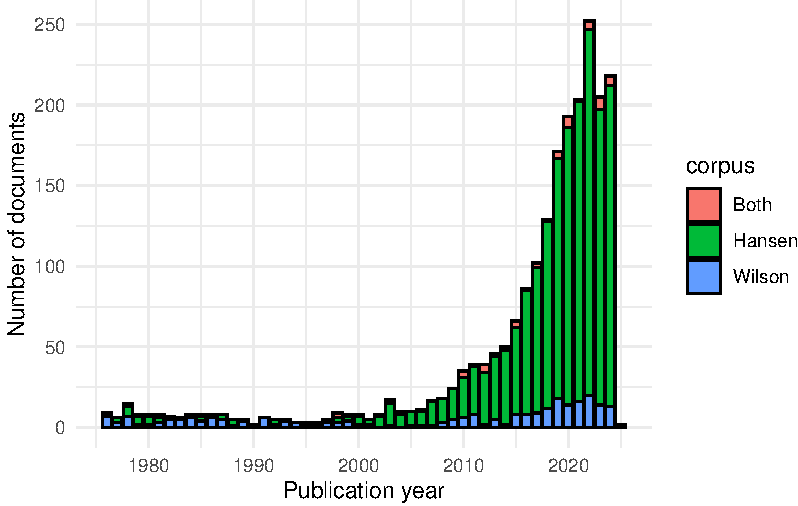
\includegraphics[width=0.7\textwidth,height=\textheight]{manuscript_files/figure-pdf/fig-docs-per-year-1.pdf}

}

\caption{\label{fig-docs-per-year}Historical pattern of publication:
documents per year.}

\end{figure}%

To illustrate this point, we conducted a bibliographic analysis of the
literature that cites Hansen (1959), Wilson (1971), or both. We
retrieved all relevant documents using the Web of Science ``Cited
References'' functionality, and the digital object identifiers of Hansen
(1959) and Wilson (1971). As a result of this search, we identified
1,788 documents that cite Hansen (1959), only 258 documents that cite
Wilson (1971), and 76 that cite both. The earliest document in this
corpus dates to 1976 and the most recent is from 2025. The number of
documents per year appears in Figure~\ref{fig-docs-per-year}, where we
see the frequency of documents over a span of almost fifty years. In
particular, we notice the remarkable growth in the number of papers that
cite Hansen (1959) compared to those that cite Wilson (1971) since the
year 2000.

As noted, literature that cites both Wilson (1971) and Hansen (1959) are
sparse (only 3.6\% of the corpus, visualised in pink in
Figure~\ref{fig-docs-per-year}). After reading the works, we can also
discern that they too are divergent, with one stream focused on
developing accessibility (i.e., \emph{potential for} spatial
interaction) and another on spatial interaction. The focuses of these
divergent streams contribute this paper's broader hypothesis that the
concepts of accessibility and spatial interaction have remained largely
disconnected, and at times, improperly conflated.

On one hand, the stream of literature focused on spatial interaction
models inspired by Wilson (1971) and which cite both Hansen (1959) and
Wilson (1971), tends to contribute to understanding how accessibility is
interpreted and incorporated in spatial interaction models. These works
treat separate spatial interaction and accessibility as a seperate but
related phenomenon. Specifically, some early works interpret the spatial
interaction model's balancing factors
(Equation~\ref{eq-production-constrained-balancing-factor} or
Equation~\ref{eq-doubly-constrained-balancing-factors}) as the inverse
of Hansen (1959)`s model (B. Harris and Wilson 1978; G. Leonardi 1978;
A. Stewart Fotheringham 1981; A. S. Fotheringham 1985), recognizing it
as a ``common sense'' approach (Morris, Dumble, and Wigan 1979, 99) to
including accessibility in the spatial interaction model, though further
exploration of its relationship is warranted (M. Batty and March 1976).
Some authors have explored this relationship, for instance as in A. S.
Fotheringham (1985) who demonstrates how the spatial interaction model
may insufficiently explain spatial patterns, and suggests that
explicitly defining destinations' accessibility as a variable within the
model may remedy the issue (e.g., the \emph{competition destination}
model). Other works used both Hansen (1959) and Wilson (1971)'s
framework in conjunction, such as in defining location-allocation
problems in operations research (G. Leonardi 1978; Beaumont 1981),
estimating trip flows (or some other spatial interaction flows)
alongside accessibility (e.g., Clarke, Eyre, and Guy 2002; Grengs 2004;
Türk 2019), or considering accessibility within spatial interaction
models, in line with A. S. Fotheringham (1985)'s demonstration (e.g.,
Beckers et al. 2022). Other works departed from Hansen (1959)'s
definition and aligned with spatial interaction in different ways, such
as using micro-economic consumer behaviour concepts to express potential
for spatial interaction (Morris, Dumble, and Wigan 1979; Giorgio
Leonardi and Tadei 1984).

On the other hand, there is another subset of literature that cite both
Hansen (1959) and Wilson (1971) that is accessibility-focused. We
categorise their citation of Wilson (1971) for three general reasons.
Firstly, a group of these works cite Wilson (1971) as attribution for
using context-dependent travel cost functions (e.g., Weibull 1980; S. L.
Handy and Niemeier 1997; Kwan 1998; Q. Shen 1998a; Ashiru, Polak, and
Noland 2003; Rau and Vega 2012; Pan 2013; Margarida Condeço Melhorado et
al. 2016; Caschili, De Montis, and Trogu 2015; Grengs 2015; Pan, Jin,
and Liu 2020; Chia and Lee 2020; Roblot et al. 2021; Sharifiasl, Kharel,
and Pan 2023; Kharel, Sharifiasl, and Pan 2024). These works do not
necessarily comment on spatial interaction explicitly. Secondly, another
group of this accessibility-focused ``both'' citing literature
\emph{does} associate spatial interaction as defined in Wilson (1971)
with accessibility's potential for spatial interaction more explicitly
(e.g., H. J. Miller 1999; Giuliano et al. 2010; Grengs et al. 2010;
Grengs 2010, 2012; Levine et al. 2012; Levinson and Huang 2012; Tong,
Zhou, and Miller 2015; X. Liu and Zhou 2015; He et al. 2017; Wu and
Levinson 2020; Ng et al. 2022; Naqavi et al. 2023; Suel et al. 2024). We
agree accessibility and spatial interaction are related topics:
accessibility is an expression of its \emph{potential} and the Wilson
(1971) paper briefly touches on the concept. However, in some of this
literature, Hansen (1959) and Wilson (1971) are co-cited as both being
`gravity models' (e.g., S. Liu and Zhu 2004; Dai, Wan, and Gai 2017; Y.
Shen 2019; Chia and Lee 2020), perhaps revealing the murkiness of the
distinction between spatial interaction and the \emph{potential for}
spatial interaction in the literature. Thirdly, there is a group of
accessibility-focused works that interpret Hansen (1959)'s model as the
singly- or doubly- constrained spatial interaction model's inverse
balancing factor (e.g., R. W. Vickerman 1974). This group cities the
earlier spatial interaction works that make this connection and is
especially prominent in the investigation of competitive accessibility
topics (e.g., Karst and Van Eck 2003; Karst T. Geurs, van Wee, and
Rietveld 2006; Willigers, Floor, and van Wee 2007; El-Geneidy and
Levinson 2011; Curtis and Scheurer 2010; Manaugh and El-Geneidy 2012;
Chen and Silva 2013; Alonso et al. 2014; Albacete et al. 2017;
Sahebgharani, Mohammadi, and Haghshenas 2019; Mayaud et al. 2019; Allen
and Farber 2020; Levinson and Wu 2020; Marwal and Silva 2022; Su and
Goulias 2023). As outlined in preceding sections, we argue interpreting
the singly- or doubly- constrained spatial interaction model's balancing
factor as accessibility yields output values that are similarly plagued
by interpretability issues.

Lastly, as an extension of the third reason within this group, only the
works of Soukhov et al. (2023) and Soukhov et al. (2024) use Wilson
(1971)'s balancing factors as a method for maintaining constraints on
opportunities within the context of competitive accessibility. These
works introduce the balancing factors as a mechanisms to ensure that
opportunities at each destination are proportionally allocated to each
zone (based on the proportion of population seeking opportunities and
the relative travel impedance). This is to ensure that each zonal
accessibility value is the sum of this proportional allocation from each
destination, and that all zonal values ultimately sum to the total
number of opportunities in the region. However, these balancing factors
were deduced intuitively. These works do not explicitly state that the
mathematical formulation of the equations are effectively equivalent to
Wilson's singly constrained model (derived from entropy maximization).
This equivalence is only discovered in hindsight, as will be
demonstrated in this study. These two works also do not discuss other
constrained cases that will be addressed in the next section.

\section{A family of accessibility
measures}\label{a-family-of-accessibility-measures}

In this section, we introduce a family of accessibility measures
inspired by Wilson's spatial interaction modelling framework. At the end
of this section, Table 8 presents a summary, where each member of the
family of accessibility measure is explained in plain language,
alongside their balancing factor, proportional allocation factor and
mathematical equation and value interpretations.

As argued in the preceding section, the streams of research on
accessibility and spatial interaction modelling have evolved as largely
separate streams with little contact since Hansen (1959) and Wilson
(1971). This may explain why the constraints and associated balancing
factors of spatial interaction models did not cross over to
accessibility analysis. This is intriguing since Wilson made an effort
to connect developments in spatial interaction modelling to
accessibility, noting for instance, the denominator of the
proportionality constants specific to origins
(Equation~\ref{eq-production-constrained-balancing-factor}) is the
inverse of balancing factor \(A_i\) (Wilson 1971, 10):

\begin{equation}\phantomsection\label{eq-Ai-as-accessibility}{
S_i = \frac{1}{A_i} = \sum_j W_j^{(2)} f(c_{ij})
}\end{equation}

Understanding \(S_i\) as the inverse of Wilson's \(A_i\) does not
uncover any new meaning for \(S_i\) itself. Indeed, mathematically it is
true, \(A_i\)'s role in Wilson's general model
\(T_{ij} = k W_i^{(1)} W_j^{(2)} f(c_{ij})\) is that of a balancing
factor \(k\) i.e., keeping units balanced and proportionality based on
constraints. Understanding \(S_i\) itself as a balancing factor is not
wholly helpful as Hansen and (Stewart before him) defined accessibility
as a partial sum of the demographic force \(F\) or the system-wide
population potential of opportunities for spatial interaction (i.e.,
(\textbf{q-stewart-population-potential-sum?}) representing
\(V_i = \sum_j \frac{M_j}{d_{ij}}\) after losing \(G\)).

Hence, we propose stepping back to introduce a revised definition of
accessibility: the \emph{constrained} potential for spatial interaction.
Once we bring back Wilson's proportionality constant \(k\) into the
picture, we can define the \emph{potential for spatial interaction}
between two locations \(i\) and \(j\) is as follows:

\begin{equation}\phantomsection\label{eq-access-01}{
V_{ij} = k W_j^{(2)} f(c_{ij})
}\end{equation}

\noindent where \(V_{ij}\) is the potential for interaction from \(i\)
to \(j\). The accessibility from origin \(i\) can then be summarised as
as a partial sum of the potential at \(i\):

\begin{equation}\phantomsection\label{eq-accesssibility-01}{
V_{i} = k \sum_j W_j^{(2)} f(c_{ij})
}\end{equation}

Similar to Equation~\ref{eq-phys-gravity-model}, \(W_j^{(2)}\) above is
the mass at the destination and the sub-indices are for
\(i = 1,\cdots, n\) origins and \(j = 1,\cdots, m\) destinations.

The market potential variant can also be generally defined, which is
effectively the transpose of \(i\) and \(j\) in
Equation~\ref{eq-access-01} and Equation~\ref{eq-accesssibility-01} as
follows: \begin{equation}\phantomsection\label{eq-market-01}{
M_{ji} = k W_i^{(1)} f(c_{ij})
}\end{equation}

\begin{equation}\phantomsection\label{eq-market-potential-01}{
M_{j} = k \sum_j W_i^{(1)} f(c_{ji})
}\end{equation}

Similar to Equation~\ref{eq-phys-gravity-model}, \(W_j^{(2)}\) above is
the mass at the destination and the sub-indices are for
\(i = 1,\cdots, n\) origins and \(j = 1,\cdots, m\) destinations.

To detail the anatomy of \(V_{ij}\) and \(M_{ji}\) along with the
partial sums of \(V_i\) and \(M_j\), Figure
Figure~\ref{fig-analytical-device-conc-accessibility} illustrates the
accessibility analytical framework we propose using a simple 3 zone
system. Each measure's most disaggregate value is \(X_{ij}\), potential
for spatial interaction from \(i\) to \(j\). The \(X\) is a stand in for
the \(ij\) values of all the cases and their variants that will be
described (i.e.,
\(V_{ij}^0, M_{ji}^0, V_{ij}^T, M_{ji}^T, V_{ij}^S, M_{ji}^S\) and
\(V_{ij}^D, M_{ji}^D\)). The single marginals represent the origin-side
and destination-side weights of the zones. The total marginal represent
the sum of a single marginal.

\begin{figure}[H]

\centering{

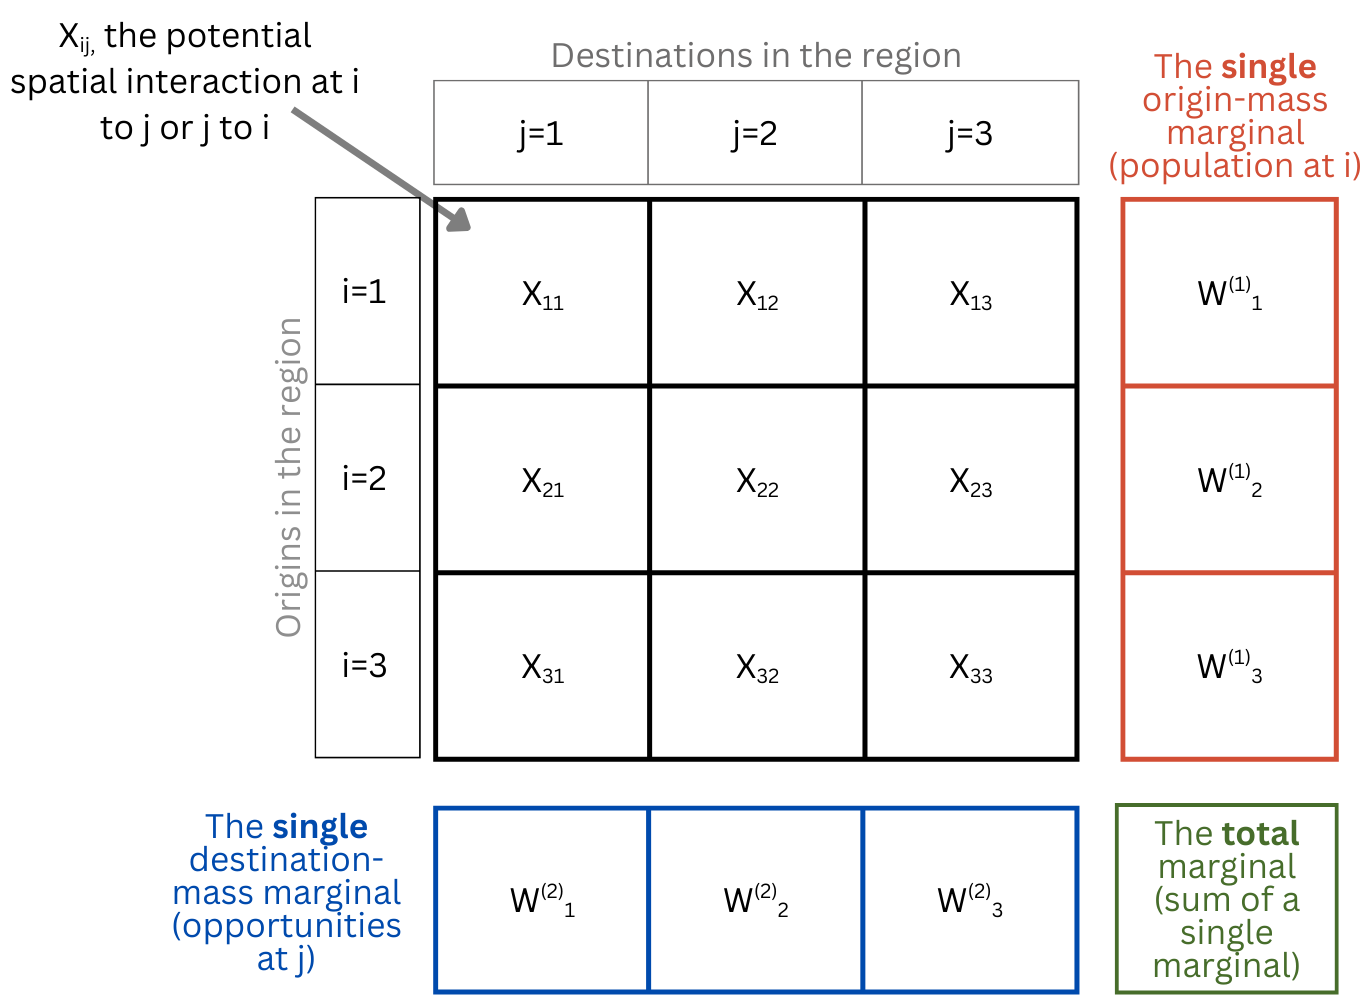
\includegraphics[width=0.7\textwidth,height=\textheight]{../figures/access-analytical-device.png}

}

\caption{\label{fig-analytical-device-conc-accessibility}The family of
accessibility measures analytical framework: labelling and associating
ij flows, zonal weights, the single marginals, and the total marginal.}

\end{figure}%

As an additional overview, we define four distinct members of the
constrained accessibility measure family, all delineated based on their
constant \(k\), which takes the form of either balancing factors
\(K^T\), \(B_j\), \(A_i\) depending on the indicator:

\begin{enumerate}
\def\labelenumi{\arabic{enumi}.}
\item
  \textbf{The unconstrained case} with variants \(V_i^0\) and \(M_i^0\).
  This case is equivalent to Hansen (1959)`s formulation (first variant)
  and Reilly (1929)'s market potential formulation (second variant),
  whereby a balancing factor is neglected, so units of zonal values are
  in units of 'opportunities-by-travel-impedance-value' and
  `population-by-travel-impedance-value'. In this case, no constraints
  are introduced to ensure that values of marginals are preserved.
\item
  \textbf{The total constrained case} with variant \(V_i^T\) and variant
  \(M_j^T\). The first variant \(V_i^T\)--the \emph{total constrained
  accessible opportunities measure}--resembles Hansen (1959)`s
  formulation but with an additional regional balancing factor \(K^T\)
  term, defined as the ratio of the total number of opportunities in the
  region to the total sum of unconstrained accessibility values in the
  region. In this way, \(K^T\) ensures that each zonal accessibility
  value is a proportion of the total opportunities in the region (i.e.,
  the total marginal in
  Figure~\ref{fig-analytical-device-conc-accessibility}), requires no
  information about the population seeking opportunities, and is in
  units of 'opportunities' accessible. The second variant \(M_j^T\) is
  the transpose of \(i\) to \(j\) of the first variant, effectively a
  constrained version of market potential and is referred to as
  \emph{total constrained accessible population measure}. In this
  variant, each zonal accessibility value is a proportion of the total
  population in the region (maintained by \(\hat K^T\)), requires no
  information about the opportunities that are sought, and each zonal
  value is in units of `population' accessible.
\end{enumerate}

\begin{itemize}
\tightlist
\item
  When conceptualising \emph{potential} for spatial interaction--whether
  with opportunities or population--the total constrained case reflects
  the lowest level of restriction and hence maximum potential. The
  balancing factors \(K^T\) and \(\hat K^T\) only ensure that
  \(V_{ij}^T\) and \(M_{ji}^T\) values end up matching the \emph{total
  sum} of one of the single marginals, not the individual marginals
  themselves. For example, \(K^T\) does not guarantee that all the
  opportunities accessibility at \(V_{i=1}^T\) reflect a proportional
  allocation of the destination mass (i.e., \emph{number} of
  opportunities) at \(j=1, 2, 3\). In some cases, an allocation of
  opportunities from a destination \(j\) to \(i=1\) could \emph{exceed}
  the number of opportunities at that \(j\) (i.e., meaning that
  destination \(j\) is very attractive and reachable for an \(i\),
  relative other flows in the region). However, what \(K^T\) \emph{does}
  ensure is that each \(V_{ij}^T\) does not exceed the overall number of
  opportunities in the region--the total marginal. In other words,
  \(V_{i=1}^T\) expresses the number of opportunities that origin
  \(i=1\) could potentially interact with, as drawn from the entire
  regional opportunity mass, rather than constrained by individual
  destination totals. In this way, the \emph{total constrained} case
  reflects the maximum amount of \emph{potential} while still
  maintaining interpretable units.
\end{itemize}

\begin{enumerate}
\def\labelenumi{\arabic{enumi}.}
\setcounter{enumi}{2}
\tightlist
\item
  \textbf{The singly constrained case}, with two variants \(V_i^S\)
  (opportunity-constrained) and \(M_j^S\) (population-constrained). The
  first variant is mathematically equivalent to the spatial availability
  measure (Soukhov et al. 2023), and this variant's per capita form is
  equivalent to the popular 2SFCA measure (Luo and Wang 2003; Q. Shen
  1998b). Both variants can also be defined using either Hansen (1959)'s
  or the market potential formulation but with balancing factor \(B_j\)
  for \(V_i^S\) or \(A_i\) for \(M_j^S\). These balancing factors ensure
  that the total marginal (green box in
  Figure~\ref{fig-analytical-device-conc-accessibility}) is maintained
  \emph{as well as} the values at one of the single marginals
  (destination-mass marginal for opportunity-constrained and origin-mass
  marginal for population constrained in
  Figure~\ref{fig-analytical-device-conc-accessibility}). In this way,
  the singly constrained case reflects a medium amount of potential,
  restricted by either values fitting the single destination-mass
  marginal or the single origin-mass marginal.
\end{enumerate}

\begin{itemize}
\tightlist
\item
  The first variant \(V_i^S\) includes a set of destination-side
  balancing factors \(B_j\) which ensure opportunities (or destination
  masses) are allocated to each origin \(i\) based on the population
  (i.e, origin mass) of the origin \(i\) and travel impedance from that
  \(j\) to all \(i\)s. Hence, \(B_j\) ensures that each \(V_i^S\) is the
  product sum of a \emph{proportional share} of opportunities allocated
  from each destination \(j\) implicitly also being a share of the total
  opportunities in the region. Similar to the total constrained case,
  each \(V_i^S\) and \(V_ij^S\) accessibility value is expressed in
  units of `opportunities' accessible. But unlike the total constrained
  case, the singly constrained case explicitly incorporates population
  by allocating a balanced share of a destination's total opportunities
  to populations at reachable origins.
\item
  The second variant \(M_j^S\) includes a set of opportunity-side
  balancing factors \(A_i\) which ensure population (or origin masses)
  are allocated to each destination \(j\) based on the destination mass
  of the destination \(j\) and all possible travel impedance from that
  \(i\) to all \(j\)s. \(A_i\) ensures similar, but transposed, so
  constraints are satisfied. Specifically, each \(M_j^S\) represents
  both a share of the total regional population and the sum of balanced
  proportions of population from all origins, allocated to each
  destination based on the opportunities sought and travel impedance.
  Each zonal value is expressed in units of `population' accessible.
\end{itemize}

\begin{enumerate}
\def\labelenumi{\arabic{enumi}.}
\setcounter{enumi}{3}
\tightlist
\item
  \textbf{The doubly constrained case}. It is constrained simultaneously
  by population (origin masses) and opportunities (destination masses),
  so each \(V_{ij}^D\) (equivalent to \(M_{ji}^D\)) is expressed in
  units of `population-opportunity capacity' that is accessible between
  \(i\) to \(j\). This case requires the number of opportunities and
  population to match, e.g., the analyst must know the matching spatial
  interaction capacity of the population (demand) and opportunities
  (supply). By using this one-to-one matching data and the double
  constraints (i.e., \(A_i\) and \(B_j\) at once, ensuring both the
  double constraint maintains both marginals in
  Figure~\ref{fig-analytical-device-conc-accessibility}), this case
  restricts the \emph{potential} to spatially interact completely. In
  other words, the doubly constrained accessibility values reflect the
  number of predicted interactions between the opportunities and
  population, effectively, this case is equivalent formulaically as
  Wilson's doubly constrained spatial interaction model (i.e.,
  \emph{attraction-production constrained}). It can be understood as
  predicting a value of `access', and not accessibility.
\end{enumerate}

And as a summary: each member of the family of accessibility measure is
named, explained in plain language, alongside their balancing factor(s),
proportional allocation factor(s), and mathematical equation and value
interpretations in Table 1.

{\tiny
\begin{longtable}{|p{2.5cm}|p{2.5cm}|p{2.5cm}|p{3cm}|p{3cm}|}
\hline
\textbf{Name of Member and Variant} & \textbf{Constraint Explanation and Balancing Factor} & \textbf{Proportional Allocation Factor} & \textbf{Measure Equation} & \textbf{Interpretation} \\
\hline
\endfirsthead

\hline
\textbf{Name of member and Variant} & \textbf{Constraint Explanation and Balancing Factor} & \textbf{Proportional Allocation Factor} & \textbf{Measure Equation} & \textbf{Interpretation} \\
\hline
\endhead

Unconstrained Accessible Opportunities ($V_i^0$) and Unconstrained Accessibile Population ($M_j^0$)
& No constraints; marginals not equal to any regional or zonal knowns.
& None
& $V_i^0 = \sum_j D_j f(c_{ij})$;

$M_j^0 = \sum_i O_i f(c_{ij})$

& Values in various units depending on the impedance and destination-mass (e.g., "opportunities x decay") for $V_i^0$ andimpedance and origin-mass (e.g., "population x decay"); no total or marginal constraint \\
\hline

Total Constrained Accessible Opportunities ($V_i^T$) and Total Constrained Accessibile Population ($M_j^T$)
& Balancing factors $K^T$ and $\hat{K}^T$ ensures the sum of $ij$ values equals the total marginal, where:

$K^T = \frac{D}{\sum_i V_i^0}$;

$\hat{K}^T = \frac{O}{\sum_j M_j^0}$

& Allocates the total marginal as opportunities based on $\kappa_{ij}^T = K^T f(c_{ij})$ and as population based on  $\hat{\kappa}_{ji}^T = \hat K^T f(c_{ij})$

& $V^T_i =  \sum_j \kappa_{ij}^T W^{(2)}_j$;

$M_j^T =  \sum_i \hat{\kappa}_{ji}^T W^{(1)}_i$


& Values reflect a share of total regional opportunities ($V^T_i$) or population ($M^T_j$). \\
\hline

Singly Constrained Accessible Opportunities ($V_i^S$) and Singly Constrained Accessible Population ($M_j^S$)
& Single balancing factor $B_j$ (for $V_i^S$) that ensures the destination-mass marginal is constrained, and $A_i$ (for $M_j^S$) ensures the origin-mass marginal is constrained:

$B_j = \frac{1}{\sum_i W_i^{(1)} f(c_{ij})}$;

$A_i = \frac{1}{\sum_j W_j^{(2)} f(c_{ij})}$

& Allocates the single opportunities marginal proportionally based on $\kappa^S_{ij} =  B_j W_i^{(1)} f(c_{ij})$ in the case of $V_i^S$ and the single population marginal proroportionally based on $\hat \kappa^S_{ji} = A_i W_j^{(2)} f(c_{ij})$ in the case of $M_j^S$.

& $V^S_i = \sum_j \kappa^S_{ij} D_j$;

$M_j^S =  \sum_i \hat \kappa^S_{ji} O_i$

& $V^S_i$ values reflect a share of the opportunities at each destination based on origin population 'demand' and impedance; $M^S_j$ values reflect a share of the population at each origin based on destination opportunities 'supply' and impedance.\\
\hline

Doubly Constrained Access ($V_{ij}^D$ or $M_{ij}^D$)
& Values reflect both single marginals simutaneously, maintained via $A_i$ and $B_j$.
& —
& $V_{ij}^D = A_i B_j O_i D_j f(c_{ij})$
& The spatial interactions between population and opportunities (i.e., access). \\
\hline

\end{longtable}
}


Table 1: Summary of constrained accessibility measure types and
interpretations

\subsection{Setup of the simple numeric
example}\label{setup-of-the-simple-numeric-example}

Consider a simple region as shown in
Figure~\ref{fig-analytical-device-conc-accessibility}, with zone IDs 1,
2 and 3. Each zone is both an origin \(i\) and a destination \(j\). The
following three pieces of information are defined: zonal population and
opportunities, zonal cost matrix, and travel impedance functions for
three types of travel behaviour. In this example, the population are
people, the opportunities are physicians, and the region can be
described by three possible travel behaviours.

Firstly, Table~\ref{tbl-small-system-land-use} summarises the population
(in units of 10,000s of people) and the opportunities (the number of
physicians) per zone. {[}\^{}1{]}. Considering
Table~\ref{tbl-small-system-land-use}'s values, the
Provider-to-Population-Ratio (PPR) in this system is 24.5. For
reference, the number of physicians per 10,000 in Canada in 2022 was
24.97 (WHO 2025). Secondly, to pair the zonal population and opportunity
information, the assumed cost of movement (in minutes of travel time)
between origins and destinations is as shown in
Table~\ref{tbl-small-system-cost}.

\begin{table}

\caption{\label{tbl-small-system-land-use}Simple system with three zones
(ID 1, 2 and 3). Population is in 10,000 persons and opportunities in
number of physicians.}

\centering{

\fontsize{7.5pt}{9.0pt}\selectfont
\begin{tabular*}{\linewidth}{@{\extracolsep{\fill}}rcc}
\toprule
ID (i or j) & Population\textsuperscript{\textit{1}} & Opportunities\textsuperscript{\textit{2}} \\ 
\midrule\addlinespace[2.5pt]
1 & 4 & 160 \\ 
2 & 10 & 150 \\ 
3 & 6 & 180 \\ 
\bottomrule
\end{tabular*}
\begin{minipage}{\linewidth}
\textsuperscript{\textit{1}}Population is \emph{Wi\textsuperscript{(1)}} when used as a proxy for the mass at the origin, and \emph{Oi} when used as a constraint.\\
\textsuperscript{\textit{2}}Opportunities is \emph{Wj\textsuperscript{(2)}} when used as a proxy for the mass at the destination, and \emph{Dj} when used as a constraint.\\
\end{minipage}

}

\end{table}%

\begin{table}

\caption{\label{tbl-small-system-cost}Cost matrix for system with three
zones (travel time in minutes).}

\centering{

\fontsize{7.5pt}{9.0pt}\selectfont
\begin{tabular*}{\linewidth}{@{\extracolsep{\fill}}cccc}
\toprule
 & \multicolumn{3}{c}{Destination ID} \\ 
\cmidrule(lr){2-4}
Origin ID & 1 & 2 & 3 \\ 
\midrule\addlinespace[2.5pt]
1 & 10 & 30 & 15 \\ 
2 & 30 & 10 & 25 \\ 
3 & 15 & 25 & 10 \\ 
\bottomrule
\end{tabular*}

}

\end{table}%

From both Table~\ref{tbl-small-system-land-use} and
Table~\ref{tbl-small-system-cost}, Zone 3 and 1 can be interpreted as of
an urban core with major healthcare institutions and a healthcare
cluster on the edge of the city respectively, each with a moderate
residing population (with zone 3 having both a higher population and
physician count). Zone 2, can be interpreted as a more distant bedroom
community, with a relatively high population and fewer physicians. In
sum, Zones 1 and 3 are more proximate to each other than to Zone 2, and
together match Zone 2's population while offering more than twice the
physician availability.

And lastly, in Equation~\ref{eq-travel-behaviour-scenarios} we
distinguish accessibility measure values for the following three
impedance functions that represent the potential for spatial interaction
travel behaviour of the population to opportunities. Accessibility will
be calculated three times for each case, one assuming the most decay
(\(f_1(c_{ij})\)), another assuming medium decay (\(f_2(c_{ij})\)), and
a third assuming the least decaying travel behaviour (\(f_3(c_{ij})\))
for the entire region. A helpful analogy may be tying travel behaviour
to the used mode's mobility potential, i.e., the most decaying travel
behaviour (\(f_1(c_{ij})\)) would assume all travel in the region being
done by foot, while calculating accessibility assuming the least decay
(\(f_3(c_{ij})\)) would assume unfettered automobility. Or
alternatively, these functions could represent travel behaviour on
snowstorm-affected day (\(f_1(c_{ij})\)) for the entire region versus a
clear, ideal travel day (\(f_3(c_{ij})\)). As an example of a discussion
on how travel behaviour has been considered in accessibility measures
cost of travel see Paez, Scott, and Morency (2012).

\begin{equation}\phantomsection\label{eq-travel-behaviour-scenarios}{
\begin{array}{l}
f_1(c_{ij}) = \frac{1}{c_{ij}^3}\\
f_2(c_{ij}) = \frac{1}{c_{ij}^2}\\
f_3(c_{ij}) = \frac{1}{c_{ij}^{0.1}}
\end{array}
}\end{equation}

Any set of concepts representing population, opportunities, and their
associated travel behaviour, whether representing the entire region
uniformly (as we will demonstrate) or representing specific subgroups,
can be substituted into our simple example, depending on the research
question. The purpose of the following simple example is to demonstrate
the calculation of each member of the accessibility measure family,
interpret the values, and compare them both within and across travel
behaviour groups and members of the family of accessibility measures.

\subsection{Unconstrained
accessibility}\label{unconstrained-accessibility}

Setting the balancing factor \(k\) to 1 or omitting it completely in
Equation~\ref{eq-access-01} results in the unconstrained accessibility
case:

\begin{equation}\phantomsection\label{eq-unconstrained-access}{
V^0_{ij} = 1 *W_j^{(2)} f(c_{ij})
}\end{equation}

In this case, the partial sum of spatial interaction is simply identical
to Hansen's accessibility \(S_i\) (Hansen 1959), the current standard
practice in accessibility measurement:

\begin{equation}\phantomsection\label{eq-unconstrained-accessibility}{
V^0_i = \sum_j V^0_{ij} = \sum_j W^{(2)}_jf(c_{ij}) = S_i
}\end{equation}

The sum of the unconstrained accessibility values for each origin
\(V^0_{i}\) generally does not equal the total number of opportunities
\(O\) (e.g., \(\sum_i V^0_{i} \not= O\)), since arbitrarily setting
\(k\) to 1 (or neglecting \(k\) all together) strips the values of any
meaningful unit-based interpretation, the units are in `summed
opportunities by some travel impedance value'. Moreover, comparisons of
these \(V^0_{i}\) values across different contexts such as different
impedance functions \(f(c_{ij})\) or varying number of zones exacerbates
this issue as the units between \(V^0_{i}\) values change i.e.,
comparisons between a value of `summed opportunities by a travel
impedance value' to a value of `summed opportunities by another travel
impedance value' are not directly interpretable. From this perspective,
the raw unconstrained accessibility scores are not intuitively
comparable across different contexts and decay functions. They should
more appropriately be used as an ordinal variable to make comparisons of
size (i.e., greater than, less than, equal to), not to calculate ratios
or intervals (i.e., the magnitude of differences).

Returning to our numeric example, the calculated unconstrained
accessibility \(V^0_{i}\) for each origin, a sum of all the travel
impedance weighted opportunities at each destination
(\(\sum_i V^0_{i}\)), in displayed in
Table~\ref{tbl-simple-example-unconstrained-accessibility}.

\begin{table}

\caption{\label{tbl-simple-example-unconstrained-accessibility}Simple
system: unconstrained accessibility.}

\centering{

\fontsize{7.5pt}{9.0pt}\selectfont
\begin{tabular*}{\linewidth}{@{\extracolsep{\fill}}>{\raggedright\arraybackslash}p{\dimexpr 45.00pt -2\tabcolsep-1.5\arrayrulewidth}|>{\centering\arraybackslash}p{\dimexpr 135.00pt -2\tabcolsep-1.5\arrayrulewidth}>{\centering\arraybackslash}p{\dimexpr 135.00pt -2\tabcolsep-1.5\arrayrulewidth}>{\centering\arraybackslash}p{\dimexpr 135.00pt -2\tabcolsep-1.5\arrayrulewidth}}
\toprule
 & \multicolumn{3}{>{\centering\arraybackslash}m{\dimexpr 405.00pt -2\tabcolsep-1.5\arrayrulewidth}}{V\textsubscript{i}\textsuperscript{0}} \\ 
\cmidrule(lr){2-4}
 & f\textsubscript{1} (c\textsubscript{ij}) = 1/c\textsubscript{ij}\textsuperscript{3} & f\textsubscript{2} (c\textsubscript{ij}) = 1/c\textsubscript{ij}\textsuperscript{2} & f\textsubscript{3} (c\textsubscript{ij}) = 1/c\textsubscript{ij}\textsuperscript{0.1} \\ 
\cmidrule(lr){2-2} \cmidrule(lr){3-3} \cmidrule(lr){4-4}
Origin & units: \emph{physicians-minute\^{}-3} & units: \emph{physicians-minute\^{}-2} & units: \emph{physicians-minute\^{}-0.1} \\ 
\midrule\addlinespace[2.5pt]
1 & 0.219 & 2.567 & 371.143 \\ 
2 & 0.167 & 1.966 & 363.479 \\ 
3 & 0.237 & 2.751 & 373.738 \\ 
\midrule 
\midrule 
Sum & 0.6233422 & 7.283556 & 1108.361 \\ 
\bottomrule
\end{tabular*}

}

\end{table}%

As the different impedance functions represent different travel
behaviours, comparing the raw unconstrained accessibility values across
groups is meaningless beyond notions of higher or lower. For instance,
at zone 1 the difference between the least decay (\(f_3(c_{ij})\)) and
most decay (\(f_1(c_{ij})\)) groups is 370.92, but in what units? These
two values are a product of different impedance functions, making the
comparison uninterpretable in absolute terms. Likewise, we could compare
values within the same travel behaviour scenario across different zones,
as they are in the same units, however the issue of unit
interpretability will also be apparent. Considering the most decaying
scenario \(f_1(c_{ij})\) and zone 1 (the zone with a healthcare cluster
at the edge of the city): zone 1 captures 0.0181185 fewer
physicians-minute\(^{-1}\) than zone 3 (urban core). Again, the
fundamental uninterpretability of what is a
\emph{physicians-minute\(^{-1}\)} or
\emph{opportunity-weighted-travel-impedance} unit remains.

While one could attempt to adjust the units post-calculation (e.g.,
scaling, population normalization) or select impedance functions to
facilitate comparison across scenarios (potentially at the expense of
accurately reflecting travel behavior), such adjustments may introduce
bias. Hence, the raw unconstrained accessibility values themselves are
challenging to compare due to their units. To enable more meaningful
comparison, the following sections will detail the introduction of
constraining constants to ensure consistent units across scenarios and
demonstrate results on the same numeric example.

\subsection{Total constrained
accessibility}\label{total-constrained-accessibility}

In the total constrained accessibility case, a total balancing factor
proportionally adjusts unconstrained zonal accessibility values
\(V^0_i\) based on the regional sum of \(V^0_i\) and the total
population or opportunities in the region. Alternatively, we reformulate
this case using a proportional allocation constant, which allocates
opportunities (or population) proportionally based on the the travel
impedance and the total population or opportunities in the region. In
both formulations, all zonal values become a proportion of a known
system total, be it the regional opportunities or regional population
depending on the variant.

We define two variants for this case: (a) \(V_i^T\) where accessibility
is constrained by the total number of opportunities (total constrained
accessible opportunity) and which is interpreted as Hansen's
accessibility with a constraining constant, and (b) \(M_j^T\), where
\(i\) and \(j\) of the first variant is transposed, yielding a measure
constrained by the total number of population and to be interpreted as
constrained `market potential'.

\subsubsection{Total constrained accessible opportunities: Hansen's
accessibility with a total
constraint}\label{total-constrained-accessible-opportunities-hansens-accessibility-with-a-total-constraint}

Unlike in Equation~\ref{eq-access-01}, the proportionality constant
\(k\) is retained. For the total constrained case, it is represented as
\(K^T\):

\begin{equation}\phantomsection\label{eq-total-constrained-access}{
V^T_{ij} = K^T \cdot W_j^{(2)} \cdot f(c_{ij})
}\end{equation}

In this way, the total constrained accessibility measure now becomes
Hansen's accessibility with a balancing factor \(K^T\):

\begin{equation}\phantomsection\label{eq-total-constrained-accessibility}{
V^T_i = \sum_j V^T_{ij} = K^T \sum_j W^{(2)}_jf(c_{ij}) = K^T \cdot V^0_i
}\end{equation}

Imagine that the only system known is the total number of opportunities
\(D\) in the region. Accordingly, the constant we impose in this case
ensures the regional sum of total constrained accessibility is equal to
the total number of opportunities as follows:
\begin{equation}\phantomsection\label{eq-total-constraint-accessibility}{
\sum_i V^T_{i} = \sum_i\sum_j V^T_{ij} = D
}\end{equation}

This constraint is analogous to the total constraint of
Equation~\ref{eq-constraint0-gravitymodel}, congruent with Wilson's
framework. Given the total number of opportunities in the region, we can
then substitute Equation~\ref{eq-total-constrained-accessibility} in
Equation~\ref{eq-total-constraint-accessibility} to solve for \(K^T\):

\begin{equation}\phantomsection\label{eq-total-opportunity-balancing-factor}{
K^T =\frac{D}{\sum_i\sum_j V^0_{ij}} = \frac{D}{\sum_i\sum_j W^{(2)}_jf(c_{ij})}
}\end{equation}

Which is also congruent with Wilson's framework as it comparable to the
total flow spatial interaction model (e.g., Equation 2.11 in Cliff,
Martin, and Ord (1974)). Hence, rearranging the equation to have
opportunities and the proportional constant distinctly represented, our
total constrained accessibility model is:

\[
V^T_i = K^T\sum_j W^{(2)}_jf(c_{ij}) = \sum_j W^{(2)}_j\frac{D\cdot f(c_{ij})}{\sum_i\sum_j W^{(2)}_jf(c_{ij})}
\]

Further, we can see that, since \(D\) and \(W^{(2)}_j\) are both in
units of opportunities, the proportional allocation factor for the total
constrained opportunity case \(\kappa_i^T\) is dimensionless:

\[
\kappa_i^T = \frac{\sum_j D\cdot f(c_{ij})}{\sum_i\sum_j W^{(2)}_jf(c_{ij})}
\]

\noindent and therefore \(V^T_i\) is now in the units of \(W^{(2)}_j\),
that is, the mass at the destination
(\(V^T_i = \kappa_i^T\sum_j W^{(2)}_j\)). The role of \(\kappa_i^T\) in
this reformulation of accessibility is to transform between units and to
adjust the number of opportunities accessible from \(i\) so they
represent a proportion of the total number of opportunities in the
region. \(\kappa_i^T\) then assigns opportunities in proportion to the
impedance between \(i\) and \(j\). This is why we refer to
\(\kappa_i^T\) as a proportional allocation factor. On the other hand,
the proportionality constant \(K^T\) balances the units of \(V^0_i\),
the Hansen-type accessibility values, and is an alternative expression
of the total constrained accessibility measure.

Referring back to our simple numeric example, balancing factor \(K^T\)
for the most decay travel behaviour scenario
\(f_1(c_{ij}) = 1/c_{ij}^3\) would then be:

\[
\begin{array}{l}
K^T = \frac{D}{\sum_{i}\sum_{j} W_j^{(2)} f(c_{ij})}\\
K^T = \frac{D}{\frac{W_1^{(2)}}{c_{11}^3}+\frac{W_1^{(2)}}{c_{21}^3} + \frac{W_1^{(2)}}{c_{31}^3} + \cdots + \frac{W_3^{(2)}}{c_{31}^3} + \frac{W_3^{(2)}}{c_{32}^3} + \frac{W_3^{(2)}}{c_{33}^3}
}\\
K^T = \frac{490}{0.6233422} \\
K^T = 786.085
\end{array}
\]

Using the calculated proportionality constants for all zones and
multiplying them by the unconstrained accessibility value \(V^0_i\), the
total opportunity constrained accessibility values for all zones and
different travel behaviour scenarios is presented in
Table~\ref{tbl-simple-example-total-opportunity-accessibility}.
\(\kappa_i^T\) for each zone is not shown, but can be understood to be
the unitless proportion of opportunities (of the total opportunities)
allocated to each zone based on travel impedance.

\begin{table}

\caption{\label{tbl-simple-example-total-opportunity-accessibility}Simple
system: total opportunity constrained accessibility.}

\centering{

\fontsize{7.5pt}{9.0pt}\selectfont
\begin{tabular*}{\linewidth}{@{\extracolsep{\fill}}>{\raggedright\arraybackslash}p{\dimexpr 45.00pt -2\tabcolsep-1.5\arrayrulewidth}|>{\centering\arraybackslash}p{\dimexpr 135.00pt -2\tabcolsep-1.5\arrayrulewidth}>{\centering\arraybackslash}p{\dimexpr 135.00pt -2\tabcolsep-1.5\arrayrulewidth}>{\centering\arraybackslash}p{\dimexpr 135.00pt -2\tabcolsep-1.5\arrayrulewidth}}
\toprule
 & \multicolumn{3}{>{\centering\arraybackslash}m{\dimexpr 405.00pt -2\tabcolsep-1.5\arrayrulewidth}}{V\textsubscript{i}\textsuperscript{T}} \\ 
\cmidrule(lr){2-4}
 & f\textsubscript{1} (c\textsubscript{ij}) = 1/c\textsubscript{ij}\textsuperscript{3} & f\textsubscript{2} (c\textsubscript{ij}) = 1/c\textsubscript{ij}\textsuperscript{2} & f\textsubscript{3} (c\textsubscript{ij}) = 1/c\textsubscript{ij}\textsuperscript{0.1} \\ 
\cmidrule(lr){2-2} \cmidrule(lr){3-3} \cmidrule(lr){4-4}
Origin & units: \emph{physicians} & units: \emph{physicians} & units: \emph{physicians} \\ 
\midrule\addlinespace[2.5pt]
1 & 172.065 & 172.672 & 164.080 \\ 
2 & 131.627 & 132.247 & 160.692 \\ 
3 & 186.308 & 185.081 & 165.228 \\ 
\midrule 
\midrule 
Sum & 490 & 490 & 490 \\ 
\bottomrule
\end{tabular*}

}

\end{table}%

In contrast to unconstrained accessibility \(V^0_i\), imposing a
constraint -in this case a total opportunity constraint for this
variant- allows for the comparison of differences and ratios between
regions and across different travel behaviour scenarios as well. Each
value is effectively in units of physicians, with the impedance units
already accounted for by \(\kappa_i^T\).

Considering the highest decay scenario (\(f_1(c_{ij})\)), zone 1 (a
healthcare cluster at the edge of the city) captures an intermediate
amount of physicians (172.0652825) like in the unconstrained
accessibility case. However, unlike in the unconstrained case, we can
say that this value is out of the 490 physicians in the region, which
allows us also to deduce that zone 1 captures 1.3072213 and 0.9235529
times more than zone 2 and 3. Values for the lesser decay
(\(f_2(c_{ij})\)) and lowest decay (\(f_3(c_{ij})\)) scenarios are
calculated separately, with decay scenario values also summing to equal
490 physicians accessible in the region.

One can also directly compare values at a specific zone due to the
consistent units. For instance, zone 1 remains intermediate in capturing
accessible physicians relative to zones 2 and 3 across scenarios,
similar to the unconstrained case. However, the difference between
travel behaviour scenarios differ in direction. Specifically, Zone 1
captures 0.6067946 more and 7.9850478 fewer opportunities than the
lesser decay scenarios \(f_2(c_{ij})\) and \(f_3(c_{ij})\) respectively.
Why? \(\kappa_i^T\) ensures proportional allocation for each travel
behaviour scenario. Meaning, while the unconstrained accessibility
increases, \(\kappa_i^T\) adjusts the values to remain proportional to
the total number of opportunities (490 physicians accessible in the
region). As the decay behaviour decreases, more opportunities are
accessible for all zones. In the medium decay scenario \(f_2(c_{ij})\),
zone 1 sees a slight increase in values (relative to the highest decay
scenario) as the zone can accessible more opportunities relative to
increases seen in other zones. However, in the lowest decay scenario,
zone 1 sees a decrease, as it is outpaced by increases in other zones -
namely zone 2 (recall: zone 2 has the lowest number of opportunities,
hence the increases in opportunity gains is much higher in a low decay
scenario).

Using the total opportunity constrained formulation of accessibility
offers a solution to the unit interpretability issue of Hansen (1959)'s
accessibility measure. Intuitively, the use of the constraint
illustrates how the differences and ratios of values between zones and
decay groups can be compared. This is true for other constrained cases
of the family of accessibility measures.

\subsubsection{Total constrained accessible population: Reilly's
potential trade territories with a total
constraint}\label{total-constrained-accessible-population-reillys-potential-trade-territories-with-a-total-constraint}

Another variant of the total constrained accessibility measure is the
\emph{total constrained accessible population measure}, which represents
the transpose of \(i\) to \(j\) of the total constrained accessible
opportunities measure. This variant, expressed in
Equation~\ref{eq-total-constrained-market}, represents an expression of
the concept of market potential (i.e., potential users) as proposed in
C. D. Harris (1954) and R. W. Vickerman (1974), and which Reilly earlier
referred to as `potential trade territories' (Reilly 1929). This
unconstrained form of market potential \(M_j^0\)
(Equation~\ref{eq-unconstrained-market}), effectively the \(i\) to \(j\)
transpose of \(V^0_{ij}\), has been used in recent research to express
the potentially accessible population (i.e., users) as a result of
regional transportation infrastructure investment projects (e.g.,
Gutiérrez 2001; Holl 2007; Condeço-Melhorado and Christidis 2018). Put
another way, market potential can also be thought of as a form of
\emph{passive accessibility}, indicating the number of people that can
reach each destination. However, like \(V_{ij}^0\), issues of unit
interpretability arise in \(M_j^0\)'s unconstrained form. To address
this, the constrained variant, the total constrained accessible
population measure \(M^T_{j}\), is introduced. To formulate this
variant, the total balancing factor \(K^T\) is applied to the mass of
the \emph{population} at \(i\) (\(W_i^{(1)}\)) instead of the
opportunities at \(j\).

\begin{equation}\phantomsection\label{eq-total-constrained-market}{
M^T_{ji} = \hat K^T \cdot W_i^{(1)} f(c_{ij}) = \hat K^T \cdot M_{ji}^0
}\end{equation}

\noindent with \(M_j^0\) being the \(i\) \(j\) transpose of
\(V^0_{ij}\):

\begin{equation}\phantomsection\label{eq-unconstrained-market}{
M_j^0 = W_i^{(1)} f(c_{ij})
}\end{equation}

The total constrained accessible population measure (market potential)
then becomes:

\[
M^T_j = \sum_i M^T_{ji} = \hat K^T \sum_i W^{(1)}_if(c_{ij})
\]

Where we impose the total system known as a constraint, i.e., that the
total market potential equals the total population \(O\) in the region:

\begin{equation}\phantomsection\label{eq-total-constraint-market}{
\sum_j M^T_{j} = \sum_i\sum_j M^T_{ji} = O
}\end{equation}

Substituting Equation~\ref{eq-total-constrained-market} in
Equation~\ref{eq-total-constraint-market}, and solving for \(\hat K^T\),
we obtain:

\begin{equation}\phantomsection\label{eq-total-population-balancing-factor}{
\hat K^T=\frac{O}{\sum_i\sum_i M^T_{ji}} = \frac{O}{\sum_i\sum_j W^{(1)}_i f(c_{ij})} 
}\end{equation}

The constrained market potential then takes the following form:

\[
M^T_j = \hat K^T\sum_i W^{(1)}_if(c_{ij}) = \sum_i W^{(2)}_i \frac{O \cdot f(c_{ij})}{\sum_i\sum_j W^{(2)}_if(c_{ij})}
\]

Where the following \(\hat \kappa_i^T\) proportional allocation factor
is dimensionless:

\[
\hat \kappa_i^T = \frac{\sum_i O \cdot f(c_{ij})}{\sum_i\sum_j W^{(2)}_if(c_{ij})}
\]

Returning back to the numerical example, the proportionality constant
\(\hat K^T\) is solved for each travel behaviour scenario, and the
market potential of each zone \(M^T_j\) is expressed as units of
population (e.g., the number of people accessible from each origin at
that destination) in
Table~\ref{tbl-simple-example-total-population-accessibility}.

\begin{table}

\caption{\label{tbl-simple-example-total-population-accessibility}Simple
system: total opportunity constrained accessibility.}

\centering{

\fontsize{7.5pt}{9.0pt}\selectfont
\begin{tabular*}{\linewidth}{@{\extracolsep{\fill}}>{\raggedright\arraybackslash}p{\dimexpr 67.50pt -2\tabcolsep-1.5\arrayrulewidth}|>{\centering\arraybackslash}p{\dimexpr 112.50pt -2\tabcolsep-1.5\arrayrulewidth}>{\centering\arraybackslash}p{\dimexpr 112.50pt -2\tabcolsep-1.5\arrayrulewidth}>{\centering\arraybackslash}p{\dimexpr 112.50pt -2\tabcolsep-1.5\arrayrulewidth}}
\toprule
 & \multicolumn{3}{>{\centering\arraybackslash}m{\dimexpr 337.50pt -2\tabcolsep-1.5\arrayrulewidth}}{M\textsubscript{i}\textsuperscript{S}} \\ 
\cmidrule(lr){2-4}
 & f\textsubscript{1} (c\textsubscript{ij}) = 1/c\textsubscript{ij}\textsuperscript{3} & f\textsubscript{2} (c\textsubscript{ij}) = 1/c\textsubscript{ij}\textsuperscript{2} & f\textsubscript{3} (c\textsubscript{ij}) = 1/c\textsubscript{ij}\textsuperscript{0.1} \\ 
\cmidrule(lr){2-2} \cmidrule(lr){3-3} \cmidrule(lr){4-4}
Destination & units: \emph{population in 10,000s} & units: \emph{population in 10,000s} & units: \emph{population in 10,000s} \\ 
\midrule\addlinespace[2.5pt]
1 & 5.018 & 5.447 & 6.598 \\ 
2 & 8.596 & 7.986 & 6.717 \\ 
3 & 6.386 & 6.567 & 6.684 \\ 
\midrule 
\midrule 
Sum & 20 & 20 & 20 \\ 
\bottomrule
\end{tabular*}

}

\end{table}%

Readers may note the difference in trends in accessible population
(Table~\ref{tbl-simple-example-total-population-accessibility}) and
accessible physicians (i.e., the preceding subsection,
Table~\ref{tbl-simple-example-total-opportunity-accessibility}). In
Table~\ref{tbl-simple-example-total-opportunity-accessibility}, zone 1,
2, 3 represent destinations and the accessibility values reflect the
number of accessible people from the vantage of physicians. Zone 1, in
its role as a destination, is no longer intermediately-ranked relative
to other zones; it now attracts the fewest number of people across all
three travel behaviour scenarios. However, similar to the total
constrained opportunity case, as travel decay reduces, the availability
of population begins to converge (though Zone 1 continues as the
lowest-ranked) for similar reasons. As decay reduces, the population's
travel impedance to all zones become more similar, making the relative
location of the zones less important and all people in the region more
equally accessible. Overall: like the total constrained accessible
opportunities case, this variant allows for the interpretation of both
ordinal and interval comparisons of the raw values themselves.

\subsection{Singly constrained
accessibility}\label{singly-constrained-accessibility}

Similar to the total constrained accessibility measure, the singly
constrained case includes a balancing factor that adjusts the
unconstrained zonal accessibility values \(V^0_i\) such that a
\emph{single} constraint is satisfied. Two variants are defined: (a) the
\emph{singly constrained accessible opportunities} case (an alternative
formula to spatial availability in Soukhov et al. (2023)), and (b) the
\emph{singly constrained accessible population} case, its transpose, or
singly constrained market potential.

Unlike the total constraint (i.e.,
Equation~\ref{eq-total-constraint-accessibility}), the single
constraint--as will be defined in
Equation~\ref{eq-opportunity-constraint} and
Equation~\ref{eq-population-constraint} for the first and second
variants-- incorporates additional information. In the
opportunities-accessible variant, the associated balancing factor
constrains the `potential' for spatial interaction by ensuring that only
a proportional amount of opportunities at each destination are allocated
to `demanding' origins. This allocation is informed by demand, or the
relative amount of population, and associated travel impedance
connecting the zones. In the population-accessible variant (i.e., the
\(i\) -\textgreater{} \(j\) transpose of the first variant), population
at each origin is proportionally allocated to destinations based on the
share of opportunities and travel impedance.

In both variants, the singly constrained accessibility measure
introduces population-based (or opportunity-based) competition at the
zonal level, unlike the total constraint, which more simply allocates a
fixed regional total of opportunities (or population depending on the
variant). In sum, all singly constrained zonal accessibility values are
both a proportion of the known regional opportunity (or population)
total \emph{and} a sum of a \emph{balanced} proportion of opportunities
allocated from each destinations (or population allocated from each
origin). Each zonal value remains in units of opportunities accessible
(or population accessible).

\subsubsection{Singly constrained accessible opportunities: spatial
availability}\label{singly-constrained-accessible-opportunities-spatial-availability}

To demonstrate this variant formulaically, we begin with the opportunity
constraint (Equation~\ref{eq-opportunity-constraint}) as our known piece
of information. Namely, the sum of accessible opportunities from a
destination should equal the number of opportunities \(D_j\) at that
destination. As the number of opportunities at each \(j\) are known, it
is represented as \(D_j\) instead of \(W_j^(2)\) as in the total
constrained case. This constraint should hold for all destinations in
the region. This is comparable to the single attraction-constraint
(Equation~\ref{eq-constraint2-gravitymodel}) from Wilson's framework.

\begin{equation}\phantomsection\label{eq-opportunity-constraint}{
\sum_i V^S_{ij} =  D_j
}\end{equation}

The underlying spatial interaction model is now the
attraction-constrained model in
Equation~\ref{eq-attraction-constrained-gravitymodel}, and our
accessibility measure becomes:

\begin{equation}\phantomsection\label{eq-opportunity-constrained-accessibility}{
V^S_{i} = \sum_j B_j D_j W_i^{(1)} f(c_{ij})
}\end{equation}

\noindent where \(W_i^{(1)}\) is a measure of the mass at origin \(i\)
(i.e., the opportunity-seeking population). The corresponding balancing
factor, as per Wilson, is:

\begin{equation}\phantomsection\label{eq-opportunity-constrained-proportionality-constants}{
B_j = \frac{1}{\sum_i W_i^{(1)} f(c_{ij})}
}\end{equation}

Introducing the balancing factor in
Equation~\ref{eq-opportunity-constrained-accessibility}, we obtain:

\begin{equation}\phantomsection\label{eq-opportunity-constrained-accessibility-with-balancing-factor}{
V^S_{i} = \sum_j D_j \frac{W_i^{(1)} f(c_{ij})}{\sum_i W_i^{(1)} f(c_{ij})}
}\end{equation}

Further, we define the following proportional allocation factor:

\begin{equation}\phantomsection\label{eq-opportunity-constrained-proportional-allocation-factor}{
\kappa^S_{i} = \frac{W_i^{(1)} f(c_{ij})}{\sum_i W_i^{(1)} f(c_{ij})}
}\end{equation}

After this, it is possible to rewrite
Equation~\ref{eq-opportunity-constrained-accessibility-with-balancing-factor}
as an origin summary expression of proportionally allocated known
opportunities (i.e., \(D_j\)).

\begin{equation}\phantomsection\label{eq-attraction-constrained-accessibility-with-proportional-allocation-factor}{
V^S_{i} = \kappa^S_{i} \sum_j   D_j
}\end{equation}

Soukhov et al. (2023) have shown that the role of \(\kappa^S_{i}\) is to
allocate opportunities \(D_j\) proportionally to the mass at each origin
\(i\) and the impedance between \(i\) and \(j\). As in the total
constrained opportunity case, \(\kappa^S_{i}\) is dimensionless and
\(V_i^S\) is in the units of opportunities \(D_j\). The singly
constrained accessibility measure in
Equation~\ref{eq-attraction-constrained-accessibility-with-proportional-allocation-factor}
is called spatial availability by Soukhov et al. (2023), because it
represents the number of opportunities that can be reached \emph{and}
are available, in the sense that accessible opportunities have been
proportionally allocated based on relative demand, travel impedance and
the regional total number of opportunities, i.e., spatial competition
for them has been considered. These authors also show that the following
expression (accessibility per capita) is a constrained version of the
popular two-stage floating catchment area measure of Q. Shen (1998b) and
Luo and Wang (2003):

\begin{equation}\phantomsection\label{eq-opportunity-constrained-accessibility-per-capita}{
v^S_{i} = \frac{V^S_{i}}{W^{(1)}_i}
}\end{equation}

Returning to the simple numeric example, the opportunity-constrained
case would yield the following \(B_{j}\) for \(f_1(c_{ij})\):

\[
\begin{array}{l}
B_{j} = \frac{1}{\sum_i W_i^{(1)} f(c_{ij})}\\
B_{1} =  \frac{1}{\frac{4}{10^3} + \frac{10}{30^3} + \frac{6}{15^3}} = 162.6506\\ 
B_{2} =  \frac{1}{\frac{4}{30^3} + \frac{10}{10^3} + \frac{6}{25^3}} = 94.9474\\
B_{3} =  \frac{1}{\frac{4}{10^3} + \frac{10}{25^3} + \frac{6}{10^3}} = 93.9850
\end{array}
\]

The balancing factors \(B_j\) for the \(f_2(c_{ij})\) decay group for
zones 1, 2 and 3 is 12.8571429, 8.7685113 and 10.6635071, and for
\(f_3(c_{ij})\) decay group is 0.0672461, 0.0660559 and 0.0663798. Using
these these balancing constants, we can calculate the singly constrained
opportunity accessibility:

\begin{table}

\caption{\label{tbl-simple-example-attraction-constrained-accessibility}Simple
system: singly constrained opportunity accessibility.}

\centering{

\fontsize{7.5pt}{9.0pt}\selectfont
\begin{tabular*}{\linewidth}{@{\extracolsep{\fill}}>{\raggedright\arraybackslash}p{\dimexpr 36.00pt -2\tabcolsep-1.5\arrayrulewidth}|>{\centering\arraybackslash}p{\dimexpr 108.00pt -2\tabcolsep-1.5\arrayrulewidth}>{\centering\arraybackslash}p{\dimexpr 108.00pt -2\tabcolsep-1.5\arrayrulewidth}>{\centering\arraybackslash}p{\dimexpr 108.00pt -2\tabcolsep-1.5\arrayrulewidth}>{\centering\arraybackslash}p{\dimexpr 108.00pt -2\tabcolsep-1.5\arrayrulewidth}}
\toprule
 &  & \multicolumn{3}{>{\centering\arraybackslash}m{\dimexpr 324.00pt -2\tabcolsep-1.5\arrayrulewidth}}{V\textsubscript{i}\textsuperscript{S}} \\ 
\cmidrule(lr){3-5}
 &  & f\textsubscript{1} (c\textsubscript{ij}) = 1/c\textsubscript{ij}\textsuperscript{3} & f\textsubscript{2} (c\textsubscript{ij}) = 1/c\textsubscript{ij}\textsuperscript{2} & f\textsubscript{3} (c\textsubscript{ij}) = 1/c\textsubscript{ij}\textsuperscript{0.1} \\ 
\cmidrule(lr){3-3} \cmidrule(lr){4-4} \cmidrule(lr){5-5}
Origin & Population (units: \emph{people in 10,000s}) & units: \emph{physicians} & units: \emph{physicians} & units: \emph{physicians} \\ 
\midrule\addlinespace[2.5pt]
1 & 4 & 133.469 & 122.255 & 98.848 \\ 
2 & 10 & 166.781 & 185.096 & 241.877 \\ 
3 & 6 & 189.750 & 182.650 & 149.275 \\ 
\midrule 
\midrule 
Sum & — & 490 & 490 & 490 \\ 
\bottomrule
\end{tabular*}

}

\end{table}%

Imposing the single proportional allocation factor \(\kappa^S_{i}\)
allows for the comparison of differences and ratios of the accessibility
values, like previously discussed in the total constrained accessible
opportunities case. The proportional allocation factor ensures that
resulting values are in units of \emph{physicians}, with the impedance
units already accounted for in the allocation process.

However, unlike the total constrained opportunity case, \(\kappa^S_{i}\)
reflects zonal competition based on the mass of the origin, i.e.,
population. Again, consider the highest decay scenario \(f_1(c_{ij})\).
Under this scenario, zone 1 no longer captures a medium amount of
physicians as in the total constrained opportunity case: it now captures
the fewest in the region i.e., 133.4687282 at zone 1, 166.7813387 at
zone 2, and 189.7499331 at zone 3. Why may zone 1 (healthcare cluster at
the edge of the city) capture 27\% of the physicians regionally while
this same zone captures 35\% in the total opportunity constrained case?

This difference is due to the single-opportunity factor
\(\kappa^S_{i}\)'s role in \(V_i^S\). The only inputs required in the
total-opportunity factor \(\kappa^T_i\) is the total number of
opportunities in the region \(D\) as well as the associated
opportunities at each \(j\) and travel impedance. Opportunities are
allocated to \(i\)s, regardless of the mass weights of origin. Whereas
the single opportunity constraint \(\kappa^S_{i}\) requires the
population at \(i\) as an input. In fact, \(\kappa^S_{i}\) is calculated
as the proportion of impedance-weighted population at an \(i\) to the
sum of impedance-weighted population for the entire region. Hence, since
zone 1 has the lowest population in the region, is in close proximity to
a more populated zone (zone 3, the `urban core'), and is not well
connected (in terms of travel impedance) to other zones with
opportunities, \(V_{1}^S\) values, or the number of physicians
accessible, is lowest.

Readers may also notice the change in the proportion of opportunities
drawn from different zones depending on the travel behaviour scenarios
considered. For instance, consider Zone 2 which has the highest
population. It is more evident in the \(f_3(c_{ij})\) scenario than in
higher decay scenarios that this zone does not have an exceptionally
large population for the region - Zone 2 only represents 50\% of the
population in the three zone region. In this sense, other zones are not
\emph{that} disadvantaged, and in this scenario with unfettered travel
cost, Zones 1 and 3 also take opportunities from Zone 2 (i.e., Zone 1
and Zone 3 takes 6\% and 8\% more from Zone 2 between \(f_3(c_{ij})\)
and \(f_1(c_{ij})\) scenarios hence \(\kappa_{2,2}^S\) decreases by
14\%). Zones 1 and 3 are allocated opportunities at relates similar to
their relative population size.

Readers may also notice the change in the proportion of opportunities
drawn from different zones depending on the travel behaviour scenarios
considered. For instance, Zone 2 has the highest zonal population,
representing 50\% of the 200,000 regional population. However, due to
its high relative travel distance from the other zones, its population
is less competitive in capturing opportunities in the high-decay travel
scenario (\(f_1(c_{ij})\)): Under this scenario, zone 2 captures almost
exclusively opportunities from its own zone. However, in
\(f_3(c_{ij})\), the scenario with unfettered travel cost, Zone 2
captures by far the most number of physicians. But in this scenario,
Zones 1 and 3 also take opportunities from Zone 2 (i.e., Zone 1 and Zone
3 takes 6\% and 8\% more from Zone 2 between \(f_3(c_{ij})\) and
\(f_1(c_{ij})\) scenarios hence \(\kappa_{2,2}^S\) decreases by 14\%).
Zones 1 and 3 are allocated opportunities at rates similar to their
relative population size.

In this way, the consideration of constrained accessibility \emph{per
capita} may be clarifying. Often, accessibility values are reported as
raw scores without the consideration for population. But, as we
introduced constraints, these constrained accessibility values can be
normalized using anything that is relevant to the zone. In
Table~\ref{tbl-simple-example-attraction-constrained-accessibility-per-capita},
we present per capita accessibility for the numeric example, simply in
units of number of physicians accessible per population at each zone.
Notably, these per capita rates are equivalent to the 2SFCA values.

\begin{table}

\caption{\label{tbl-simple-example-attraction-constrained-accessibility-per-capita}Simple
system: singly constrained opportunity accessibility per capita.}

\centering{

\fontsize{7.5pt}{9.0pt}\selectfont
\begin{tabular*}{\linewidth}{@{\extracolsep{\fill}}>{\raggedright\arraybackslash}p{\dimexpr 36.00pt -2\tabcolsep-1.5\arrayrulewidth}|>{\centering\arraybackslash}p{\dimexpr 108.00pt -2\tabcolsep-1.5\arrayrulewidth}>{\centering\arraybackslash}p{\dimexpr 108.00pt -2\tabcolsep-1.5\arrayrulewidth}>{\centering\arraybackslash}p{\dimexpr 108.00pt -2\tabcolsep-1.5\arrayrulewidth}>{\centering\arraybackslash}p{\dimexpr 108.00pt -2\tabcolsep-1.5\arrayrulewidth}}
\toprule
 &  & \multicolumn{3}{>{\centering\arraybackslash}m{\dimexpr 324.00pt -2\tabcolsep-1.5\arrayrulewidth}}{v\textsubscript{i}\textsuperscript{S}} \\ 
\cmidrule(lr){3-5}
 &  & f\textsubscript{1} (c\textsubscript{ij}) = 1/c\textsubscript{ij}\textsuperscript{3} & f\textsubscript{2} (c\textsubscript{ij}) = 1/c\textsubscript{ij}\textsuperscript{2} & f\textsubscript{3} (c\textsubscript{ij}) = 1/c\textsubscript{ij}\textsuperscript{0.1} \\ 
\cmidrule(lr){3-3} \cmidrule(lr){4-4} \cmidrule(lr){5-5}
Origin & Population (units: \emph{people in 10,000s}) & units: \emph{physicians per capita} & units: \emph{physicians per capita} & units: \emph{physicians per capita} \\ 
\midrule\addlinespace[2.5pt]
1 & 4 & 33.367 & 30.564 & 24.712 \\ 
2 & 10 & 16.678 & 18.510 & 24.188 \\ 
3 & 6 & 31.625 & 30.442 & 24.879 \\ 
\bottomrule
\end{tabular*}

}

\end{table}%

This simple example was constructed so that the regional average equals
24.5 physicians per 10,000 people. As distance decay decreases and
becomes \emph{relatively} uniform (all zones can reach all zones), the
effect of population drives the proportional allocation of
opportunities. Consequently, per capita accessibility values begin to
stabilise to the regional per capita average (e.g., in the lowest
distance decay \(f_3(c_{ij})\), per capita values are all around 24
physicians accessible per capita).

This trend mirrors how the accessibility values in the total constrained
opportunity case stabilises to the \(V_i^T\) regional average (e.g., the
accessible opportunities allocated to each of the three zones approaches
a third of 490 physicians, or 163.33, under the unfettered mobility
scenario \(f_3(c_{ij})\)). These patterns make intuitive sense: the
balancing factors act as regional and/or zonal averaging mechanisms. In
distance decay travel behaviour scenarios that are more relatively
uniform (i.e., low for all zones like in \(f_3(c_{ij})\)), what remains
is the relative effect of the other variables in the balancing factor.
In the total constrained case, this is the proportion of opportunities
relative to the regional opportunities, and in the case of the single
opportunity constrained case, this is the population at a zone relative
to the regional population.

\subsubsection{Singly constrained accessible population: market
availability}\label{singly-constrained-accessible-population-market-availability}

Similar to Equation~\ref{eq-total-population-balancing-factor} in
transposing the origins and destinations, we can define a \emph{singly
constrained} measure of market potential that preserves the known
population (i.e., the mass weight at the origin \(W_i^{(1)}\) is now
represented by \(O_i\)). In it's per-capita expression, i.e., equivalent
to 2SFCA, this constrained concept of market potential been used to
express ``facility crowdedness'' as in F. H. Wang (2018).

The underlying spatial interaction model is now the
production-constrained model in
Equation~\ref{eq-production-constrained-gravitymodel}, and our market
potential measure \(M^S_j\) becomes:

\begin{equation}\phantomsection\label{eq-population-constrained-accessibility}{
M^S_j = \sum_i A_i O_i W_j^{(2)} f(c_{ij})
}\end{equation}

In this case, the measure is singly constrained by the population
\emph{by origin} (i.e., \(O_i\)), like
Equation~\ref{eq-constraint2-gravitymodel} from Wilson's framework:

\begin{equation}\phantomsection\label{eq-population-constraint}{
\sum_j M^S_{ji} =  O_i \\
}\end{equation}

And the corresponding balancing factor, as per Wilson, is:

\begin{equation}\phantomsection\label{eq-population-constrained-proportionality-constants}{
A_i = \frac{1}{\sum_j W_j^{(2)} f(c_{ij})}
}\end{equation}

Following the same logic as in the preceding section on total
constrained market potential, one arrives at the following expression:

\begin{equation}\phantomsection\label{eq-production-constrained-accessibility-with-proportional-allocation-factor}{
M^S_{j} = \hat \kappa^S_{j} \sum_i  O_i
}\end{equation}

\noindent with:

\begin{equation}\phantomsection\label{eq-attraction-constrained-proportional-allocation-factor}{
\kappa^S _{j} = \frac{W_j^{(2)} f(c_{ij})}{\sum_i W_j^{(2)} f(c_{ij})}
}\end{equation}

As well, the single (population) constraint in
Equation~\ref{eq-population-constraint} ensures that the the total
constraint (e.g., \(\sum_j M^S_{j} = \sum_i\sum_j  M^S_{ji} = O\)) is
maintained.

With these constraints, \(\frac{M_j^S}{O}\) can be interpreted as the
proportion of the total population serviced by location \(j\).

For the sake of brevity, we'll move forward onto the doubly constrained
case.

\subsection{Doubly constrained
accessibility}\label{doubly-constrained-accessibility}

This accessibility case requires zonal populations and opportunities to
match one-to-one, like the doubly constrained spatial interaction model.
In this way, doubly constrained accessibility can be thought as
``access'' or simply spatial interaction (no potential).

To contextualize this point, the total and singly constrained
accessibility measures discussed thus far have used either \(O_i\),
\(D_j\), or the regional sums of either, but never both simultaneously.
For example, when opportunities \(D_j\) are used to constrain
Equation~\ref{eq-opportunity-constrained-accessibility} in the
\emph{singly constrained accessible opportunities measure}, the specific
mass of the population at origin \(i\) demanding only those
opportunities at that \(j\) is unknown. Instead, only the population at
\(i\) demanding opportunities in the region is known, and this is more
generally represented as \(W_i^{(1)}\) (as in
Equation~\ref{eq-opportunity-constrained-proportionality-constants}).
Similarly, when the population \(O_i\) is used as a constraint in
Equation~\ref{eq-population-constrained-accessibility} in the
\emph{singly constrained accessible population measure}, the mass at the
destination is given by \(W_j^{(2)}\) (also in
Equation~\ref{eq-population-constrained-proportionality-constants})
since only the mass of opportunities at each \(j\) is known and
information on what opportunities are allocated to what zone is unknown.

By contrast, the double-constrained accessibility case requires that
both populations and opportunities match. Meaning, opportunities at each
destination can be accessed by all populations, while at the same time,
the population at each origin can be accessed by all opportunities.
However, this requirement is often unintuitive in traditional
accessibility analysis. Namely, the distinction between population
(origin masses) and opportunities (destination masses) typically
represent different entities without a shared unit of measurement. On
the population side, we usually count people; on the opportunity side,
we may be referring to physicians, clinics, grocery stores, schools,
parks, or libraries. In a few cases, a one-to-one correspondence or
their own capacities at which they interact and are interacted with may
exist e.g., one person with one job. Another similar opportunity type
example is healthcare, e.g., one person and one unit of capacity, e.g.~a
vaccine shot.

A doubly constrained approach to accessibility calculation needs a
one-to-one relationships between population and opportunities to be
present. Mathematically, this model requires the simultaneous imposition
of both the population- and opportunity- constraints in the preceding
singly constrained variants (Equation~\ref{eq-opportunity-constraint}
and Equation~\ref{eq-population-constraint}), namely the sum of
population in all origins should match the sum of opportunities in all
destinations (Equation~\ref{eq-opportunity-population-equality}):

\begin{equation}\phantomsection\label{eq-opportunity-population-equality}{
\sum_i O_i = \sum_j D_j
}\end{equation}

As before, the simultaneous imposition of both constraints ensures the
total system constraint is maintained i.e., the sum of all doubly
constrained accessibility values
\(\sum_i V^D_{i} = \sum_i\sum_j  V^D_{ij} = D\) remains equal to the
total number of opportunities in the region \(O\) as shown in
Equation~\ref{eq-total-constraint-accessibility}.

As the doubly constrained accessibility measure \(V_{ij}^D\) takes the
form of the production-attraction (doubly constrained) spatial
interaction model, as shown in
Equation~\ref{eq-doubly-constrained-gravitymodel}, \(V_{i}^D\) is as
follows:

\begin{equation}\phantomsection\label{eq-doubly-constrained-accessibility}{
V_{ij}^D = A_i B_j O_i D_j f(c_{ij})
}\end{equation}

\noindent where the corresponding balancing factors \(A_i\) and \(B_j\),
as per Wilson, are:

\[
\begin{array}{l}
A_i = \frac{1}{\sum_j B_j D_j f(c_{ij})}\\
B_j = \frac{1}{\sum_i A_i O_i f(c_{ij})}
\end{array}
\]

Calibration of the two sets of proportionality constants is accomplished
by means of iterative proportional fitting, whereby the values of
\(A_i\) are initialized as one for all i to obtain an initial estimate
of \(B_j\). The values of \(B_j\) are used to update the underlying
\(V_{ij}^D\) matrix, before calibrating \(A_i\). This process continues
to update \(A_i\) and \(B_j\) until a convergence criterion is met (see
Ortúzar and Willumsen 2011, 193--95). The proportional allocation factor
\(\kappa_{ij}^D\) would then be:

\[
\kappa_{ij}^D = \sum_j \frac{1}{\sum_j B_j D_j f(c_{ij})} \frac{1}{\sum_i A_i O_i f(c_{ij})} O_i f(c_{ij})
\]

One could rewrite Equation~\ref{eq-doubly-constrained-accessibility} as
an origin summary expression of proportionally allocated opportunities:

\begin{equation}\phantomsection\label{eq-doubly-constrained-accessibility-w-paf}{
V^D_{i} = \kappa^D_{ij} \sum_j D_j
}\end{equation}

However, \(V^D_{i}\) is not wholly helpful, as it will simply equal the
origin-mass marginal. In this way, only \(V^D{ij}\) values are
interpretable. Furthermore, unlike in the total and singly constrained
cases, the doubly-constrained case does not have an interpretable per
capita version. For instance, representing \(V_{ij}^D\) per capita is
not meaningful, as the value \emph{already} matches population to
opportunities. Following this logic, the market potential form
\(M^D_{ij}\) is effectively equivalent to \(V_{ij}^D\), but can be read
with a different interpretation: i.e., the opportunities accessed from
\(j\) at an \(i\) vs.~the population accessed from \(i\) at a \(j\). The
inputs of `opportunities accessed' and `accessed population' can already
be interpreted as inherently being sensitive to both opportunities and
population.

To calculate doubly constrained accessibility, the interpretation of the
population data and the counts of the opportunity data in the numeric
example must be modified. Namely, a count of physician \emph{capacity}
per destination is needed instead of just the number of physicians, as
used to calculated total and singly constrained cases. We also must be
able to clearly state that the population is a count of people seeking
opportunities at the new capacities, i.e., the population must reflect
the \emph{capacity} of the population to interact with opportunities.

So, this adjusted simple example is summarised in
Table~\ref{tbl-small-system-land-use-doubly-constrained-case}: with the
population (in units of 10,000s of people seeking physicians) and the
opportunities (in units of 10,00s of physician-capacity) per zone. For
the population, we leave this unchanged numerically but theoretically
know that each person interacts with one physician capacity (i.e., our
opportunities with a \emph{capacity}). Hence, the number of
opportunities per destination is new: the example is modified such that
the physician-capacity at each zone is an approximately scaled version
of the number of destination-side physicians at each zone from the
unmodified example (Table~\ref{tbl-small-system-land-use}). To emphasis
the new definition of `provider' as physician capacity, the new system
PPR is simply 1, this is compared to the unmodified example which yields
system PPR of24.5. We keep the same zonal cost matrix, and travel
impedance functions for three types of travel behaviour as before
(Table~\ref{tbl-small-system-cost} and
Equation~\ref{eq-travel-behaviour-scenarios}).

\begin{table}

\caption{\label{tbl-small-system-land-use-doubly-constrained-case}Modified
simple system with three zones reflecting matched population and
opportunities. Population is in 10,000 persons and opportunities in
10,000 of physician-capacity.}

\centering{

\fontsize{7.5pt}{9.0pt}\selectfont
\begin{tabular*}{\linewidth}{@{\extracolsep{\fill}}rcc}
\toprule
ID (i or j) & Population & Opportunities \\ 
\midrule\addlinespace[2.5pt]
1 & 4 & 7 \\ 
2 & 10 & 5 \\ 
3 & 6 & 8 \\ 
\bottomrule
\end{tabular*}

}

\end{table}%

However, despite the modifications to the example, our objective remains
the same as in previous cases: to measure accessibility under different
travel behavior scenarios. Specifically, we aim to quantify the number
of \emph{potential} spatial interactions between the physician-seeking
population in each zone \(i\) to the physician capacity in a zone \(j\)
i.e., \(V_{ij}^D\). The highest decay travel behaviour scenario
(\(f_1(c_ij)\)) is presented in
Table~\ref{tbl-adjusted-small-system-land-use-doubly-constrained-case-f1cij-access-values}.

\begin{table}

\caption{\label{tbl-adjusted-small-system-land-use-doubly-constrained-case-f1cij-access-values}Doubly
constrained opportunity accessibility assuming the most decay travel
behaviour scenario in the modified simple system.}

\centering{

\fontsize{7.5pt}{9.0pt}\selectfont
\begin{tabular*}{\linewidth}{@{\extracolsep{\fill}}l|rcccc}
\toprule
 &  & \multicolumn{3}{c}{Destination ID} &  \\ 
\cmidrule(lr){3-5}
 & Origin ID & 1 & 2 & 3 & sum \\ 
\midrule\addlinespace[2.5pt]
 & 1 & 3.235859 & 0.01032226 & 0.7556568 & 4 \\ 
 & 2 & 2.132602 & 4.95932483 & 2.9044391 & 10 \\ 
 & 3 & 1.631539 & 0.03035291 & 4.3399040 & 6 \\ 
\midrule 
\midrule 
Sum & — & 7 & 5 & 8 & — \\ 
\bottomrule
\end{tabular*}

}

\end{table}%

As mentioned, accessibility values are typically interpreted as a
summary of the proportionally allocated opportunities at each \(i\).
Hence, in interpreting the doubly constrained accessibility from
Table~\ref{tbl-adjusted-small-system-land-use-doubly-constrained-case-f1cij-access-values},
\(V_i^D\) values (i.e., the sum of values at all three \(j\)
destinations for each origin \(i\)) would be 4.0018381, 9.9963656, and
6.0017963 physician-capacity accessible for Zones 1, 2 and 3
respectively. This approximately equal to the number of population at
each of these zones. Conversely, the market potential \(M_j^D\)
interpretation of these values would be 7, 5, and 8 people accessible
from Zones 1, 2 and 3 respectively, equal to the number of
\emph{opportunities} (physician-capacities accessible) at each of these
zones. Notice, the mass weight at the origin equals the mass weight of
the destination: this is precisely the function of the double
constraint. In other words, \(V_i^D\) is the number of accessed
opportunities and \(M_j^D\) is the number of population accessed. For
the other two travel behaviour, identical \(V_i^D\) and \(M_j^D\) values
are calculated, following the same logic. Hence, the usefulness of the
doubly constrained measure lies in the interpretation as \(V_{ij}^D\)
values.

For instance, differences in \(V_{ij}^D\) values between travel
behaviour scenarios are notable. These values can be directly compared
to discuss mass and distance decay impacts. Examining Zone 2 (the
bedroom community),
Table~\ref{tbl-adjusted-small-system-land-use-doubly-constrained-case-allfs-access-values-for-zone2}
demonstrates these \(i\) to \(j\) access values for this more relatively
remote, higher-populated and lower-opportunity rich zone. It can be
observed that the number of intrazonal opportunities proportionally
allocated decreases as the assumed distance decay decreases e.g., from
4.9593248 to 2.6672837 out of the \textasciitilde10 opportunities
allocated to Zone 2 (a population of 10). Following the intuition
discussed in the singly constrained opportunity case, as decay
decreases, the mass effect of the population (at origin) and opportunity
(at destination) is more evident: zonal opportunities are supplied and
zonal populations demand at the weights assigned to these zones, with
minimal decay adjustment, reflected by the proportional allocation
factors \(\kappa_{ij}^D\).

\begin{table}

\caption{\label{tbl-adjusted-small-system-land-use-doubly-constrained-case-allfs-access-values-for-zone2}Doubly
constrained opportunity accessibility for all travel behaviour scenarios
for Zone 2 in the modified simple system.}

\centering{

\fontsize{7.5pt}{9.0pt}\selectfont
\begin{tabular*}{\linewidth}{@{\extracolsep{\fill}}>{\raggedright\arraybackslash}p{\dimexpr 22.50pt -2\tabcolsep-1.5\arrayrulewidth}|>{\centering\arraybackslash}p{\dimexpr 67.50pt -2\tabcolsep-1.5\arrayrulewidth}>{\centering\arraybackslash}p{\dimexpr 67.50pt -2\tabcolsep-1.5\arrayrulewidth}>{\centering\arraybackslash}p{\dimexpr 67.50pt -2\tabcolsep-1.5\arrayrulewidth}>{\centering\arraybackslash}p{\dimexpr 67.50pt -2\tabcolsep-1.5\arrayrulewidth}>{\centering\arraybackslash}p{\dimexpr 67.50pt -2\tabcolsep-1.5\arrayrulewidth}}
\toprule
 &  &  & \multicolumn{3}{>{\centering\arraybackslash}m{\dimexpr 202.50pt -2\tabcolsep-1.5\arrayrulewidth}}{V\textsubscript{\{ij\}}\textsuperscript{D}} \\ 
\cmidrule(lr){4-6}
 &  &  & f\textsubscript{1} (c\textsubscript{ij}) = 1/c\textsubscript{ij}\textsuperscript{3} & f\textsubscript{2} (c\textsubscript{ij}) = 1/c\textsubscript{ij}\textsuperscript{2} & f\textsubscript{3} (c\textsubscript{ij}) = 1/c\textsubscript{ij}\textsuperscript{0.1} \\ 
\cmidrule(lr){4-4} \cmidrule(lr){5-5} \cmidrule(lr){6-6}
Dest. & Population at 2 (units: \emph{people in 10,000s}) & Opportunities (units: \emph{capacity in 10,000s}) & units: \emph{physician-capacity in 10,000s} & units: \emph{physician-capacity in 10,000s} & units: \emph{physician-capacity in 10,000s} \\ 
\midrule\addlinespace[2.5pt]
1 & 10.000 & 7.000 & 2.133 & 2.272 & 3.411 \\ 
2 & 10.000 & 5.000 & 4.959 & 4.766 & 2.667 \\ 
3 & 10.000 & 8.000 & 2.904 & 2.958 & 3.919 \\ 
\bottomrule
\end{tabular*}

}

\end{table}%

Recall, accessibility is defined as ``the potential for interaction''
and is traditionally presented as a summary zonal measure. In the doubly
constrained case, we force the zonal population and zonal opportunities
to match one-to-one, hence providing a zonal summary is no longer
relevant: the sum of \(V_{ij}^D\) for all \(i\)s ends up being equal to
the population at the zone. However, if what interests readers is the
``potential for interaction'' in the case population and opportunities
to match one-to-one, reframing the investigation may be needed. In this
sense, it would be examining ``interaction'' (much less room for
potential) through the values of \(V_{ij}^D\) e.g., how many
opportunities are being allocated to an origin from a destination (or in
a transposed sense for \(M_{ji}^D\)). In this sense, the doubly
constrained case can be thought of as an estimate of \emph{realized}
accessibility or access: reflecting spatial interaction. It is also
formulaically identical to the doubly constrained spatial interaction
model, but with specific interpretations of the origin and destination
weights as `population' and `opportunity', respectively.

As Wilson explicitly noted, origin and destination weights defined in
the spatial interaction model \emph{can} be defined using any unit.
Accessibility, however, is often presented and understood as a zonal
summary of \emph{potential} for interaction between origins and
destinations that contain inherently different units. Arriving at the
doubly constrained case through the unconstrained, total, and singly
constrained cases make the connection between the \emph{potential} for
spatial interaction (accessibility) and \emph{realized} potential for
spatial interaction more interpretable. Namely, by demonstrating that
these members of the accessibility family all derive from the same root
and can be derived from Wilson's original formulation, this more clearly
demonstrates what \emph{potential} is, within the context of spatial
interaction modelling.

Namely, \emph{potential} depends on the framing of the masses at the
origin and destination, and how similar they are in their units. The
appropriate constraint should be decided based on the the input data and
their similarity. In increasing unit similarity from the perspective of
opportunity-constraint: the total-constraint can be used if population
(origin mass) is not known, the single constraint can be used if
population is known and matters to \emph{potential} but it does not
match the capacity of opportunities, and lastly, the double constraint
is appropriate if population is known, matters and population matches
the capacity of opportunities. These constraint measures can reflect the
opportunities accessible at each zone, but reflects the assumptions
embedded in the input data about the potential to spatially interact.

\section{Conclusions}\label{conclusions}

In this work, we examined the historical and mathematical commonalities
between spatial interaction models and place-based accessibility
measures. As accessibility research evolved largely influenced by Hansen
(1959), researchers in the field neglected the proportionality constant
that was originally present in gravity-based models, and is still
present in spatial interaction modeling. Firstly, we have demonstrated
that by reintroducing such constraints and defining associated balancing
factors and proportional allocation factors, we can derive a unifying
family of accessibility measures that reintroduces units to the
resulting values. These values become more intuitive for the purpose of
analysis and comparison. Secondly, the constraining constants, depending
on the case (i.e., total, singly- or doubly- constrained), restrict the
degree of \emph{potential}, linking accessibility (the potential for
spatial interaction) with access (spatial interaction) on the same
continuum based on the constraint used. Lastly, we discussed how popular
measures such as the one used in Hansen (1959) and the 2SFCA link into
the family of accessibility measures. We summarise the family of
accessibility measures, as follows.

We first place the popular Hansen-type accessibility measure (Hansen
1959) within this family of measures as an ``unconstrained'' case,
demonstrating that resulting values cannot be directly compared across
different travel scenarios without ad-hoc adjustments. We then show how
applying a total constraint balances the units and produces a
statistically averaged solution that converges to the regional average
for each zone as the decay effect decreases. In other words, the
total-constraint model could be a more interpretable alternative for the
unconstrained case if population-competition is not relevant and one is
interested in capturing the maximum \emph{potential}; specifically, if
there is a fixed number of opportunities in the region, and if it makes
sense to assume that people accessing proximate opportunities leave
fewer for others, \emph{without} considering the population size at the
origins.

We then introduce the singly constrained case, which \emph{does} takes
into account the population size at the origin in the allocation of
opportunities (unlike the total constraint). It is also mathematically
equivalent to the spatial availability introduced in Soukhov et al.
(2023). In this case, all accessibility values are fixed to sum to a
known zonal opportunity-size value (implicitly, the regional total of
opportunities), but they are not required to sum to any population-based
values at the zone or regional level. The singly constrained model could
be useful if regional competition is a factor and if the acknowledgment
that only a finite number of opportunities can be allocated from each
destination (with those allocations distributed based on origin
population size) is suitable. We also introduce an `accessible' PPR
(e.g., opportunities per capita), calculated by dividing each
accessibility value by the zonal population. To clarify, this per capita
expression of the singly constrained case is equivalent to the 2SFCA
(Luo and Wang 2003; Q. Shen 1998b), hence linking this literature back
to spatial interaction principles.

Lastly, the doubly constrained case is introduced. In this case, the
sums must equal both the regional total and ensure that no zone
allocates more opportunities than it has available. Specifically,
accessibility values for each \(i\)-\(j\) pair must be a proportion of
he zonal opportunity and population values simultaneously. For example,
the accessibility at zone 1 must equal the sum of opportunities from
zones 1, 2, and 3, as well as the sum of the population at zone 1.
Satisfying the double constraint means the opportunities and population
data must match one-to-one, so working with the accessibility
\(i\)-\(j\) pair values should be of interest. In this sense, the
research question should be concerned with `access' (how many
opportunities accessed from \(j\) at \(i\) based on given zonal
opportunities and populations) instead of potential spatial interaction
(e.g., typically expressed as a zonal summary measure of how many
opportunities one could reach (out of a regional total and/or
zonal-allocation).

In summary, building on Wilson (1971)'s foundational work, this paper
proposed a unified framework for accessibility that is able to account
for competition. By reintroducing Wilson's proportionality constant, the
proposed family of constrained accessibility measures restores
measurement units to accessibility estimates. This enhancement provides
a more interpretable, consistent, and theoretically grounded basis for
accessibility analysis, which could help advance the adoption of
accessibility-oriented planning.

\section*{References}\label{references}
\addcontentsline{toc}{section}{References}

\phantomsection\label{refs}
\begin{CSLReferences}{1}{0}
\bibitem[\citeproctext]{ref-albacete2017measuring}
Albacete, Xavier, Doina Olaru, Valerià Paül, and Sharon Biermann. 2017.
{``Measuring the Accessibility of Public Transport: A Critical
Comparison Between Methods in Helsinki.''} \emph{Applied Spatial
Analysis and Policy} 10: 161--88.

\bibitem[\citeproctext]{ref-allenMeasureCompetitiveAccess2020}
Allen, Jeff, and Steven Farber. 2020. {``A Measure of Competitive Access
to Destinations for Comparing Across Multiple Study Regions.''}
\emph{Geographical Analysis} 52 (1): 69--86.
\url{https://doi.org/10.1111/gean.12188}.

\bibitem[\citeproctext]{ref-alonso2014labour}
Alonso, M Pilar, MA Beamonte, Pilar Gargallo, and Manuel J Salvador.
2014. {``Labour and Residential Accessibility: A Bayesian Analysis Based
on Poisson Gravity Models with Spatial Effects.''} \emph{Journal of
Geographical Systems} 16: 409--39.

\bibitem[\citeproctext]{ref-ashiru2003space}
Ashiru, Olu, John W Polak, and Robert B Noland. 2003. {``Space-Time User
Benefit and Utility Accessibility Measures for Individual Activity
Schedules.''} \emph{Transportation Research Record} 1854 (1): 62--73.

\bibitem[\citeproctext]{ref-battyChronicleScientificPlanning1994}
Batty, Michael. 1994. {``A {Chronicle} of {Scientific} {Planning}: {The}
{Anglo}-{American} {Modeling} {Experience}.''} \emph{Journal of the
American Planning Association} 60 (1): 7--16.
\url{https://doi.org/10.1080/01944369408975546}.

\bibitem[\citeproctext]{ref-battyMethodResiduesUrban1976}
Batty, M, and L March. 1976. {``The Method of Residues in Urban
Modelling.''} \emph{Environment and Planning A: Economy and Space} 8
(2): 189--214. \url{https://doi.org/10.1068/a080189}.

\bibitem[\citeproctext]{ref-beaumontLocationallocationProblemsPlane1981}
Beaumont, John R. 1981. {``Location-Allocation Problems in a Plane a
Review of Some Models.''} \emph{Socio-Economic Planning Sciences} 15
(5): 217--29. \url{https://doi.org/10.1016/0038-0121(81)90042-2}.

\bibitem[\citeproctext]{ref-beckers2022incorporating}
Beckers, Joris, Mark Birkin, Graham Clarke, Nick Hood, Andy Newing, and
Ryan Urquhart. 2022. {``Incorporating e-Commerce into Retail Location
Models.''} \emph{Geographical Analysis} 54 (2): 274--93.

\bibitem[\citeproctext]{ref-boisjoly2017informality}
Boisjoly, Geneviève, Ana Isabel Moreno-Monroy, and Ahmed El-Geneidy.
2017. {``Informality and Accessibility to Health by Public Transit:
Evidence from the São Paulo Metropolitan Region.''} Journal Article.
\emph{Journal of Transport Geography} 64: 89--96.
\url{https://doi.org/10.1016/j.jtrangeo.2017.08.005}.

\bibitem[\citeproctext]{ref-careyPrinciplesSocialScience1858}
Carey, Henry Charles. 1858. \emph{Principles of Social Science}.
University of Michigan Library Digital Collections: In the digital
collection Making of America Books.
\url{https://name.umdl.umich.edu/AFR1829.0001.001.}

\bibitem[\citeproctext]{ref-caschili2015accessibility}
Caschili, Simone, Andrea De Montis, and Daniele Trogu. 2015.
{``Accessibility and Rurality Indicators for Regional Development.''}
\emph{Computers, Environment and Urban Systems} 49: 98--114.

\bibitem[\citeproctext]{ref-cavendish_xxi_1798}
Cavendish, Henry. 1798. {``{XXI}. {Experiments} to Determine the Density
of the Earth.''} \emph{Philosophical Transactions of the Royal Society}
88: 469--526. \url{https://doi.org/10.1098/rstl.1798.0022}.

\bibitem[\citeproctext]{ref-chen2013regional}
Chen, Guineng, and João de Abreu e Silva. 2013. {``Regional Impacts of
High-Speed Rail: A Review of Methods and Models.''} \emph{Transportation
Letters} 5 (3): 131--43.

\bibitem[\citeproctext]{ref-chia2020extending}
Chia, Jason, and Jinwoo Brian Lee. 2020. {``Extending Public Transit
Accessibility Models to Recognise Transfer Location.''} \emph{Journal of
Transport Geography} 82: 102618.

\bibitem[\citeproctext]{ref-clarke2002deriving}
Clarke, Graham, Heather Eyre, and Cliff Guy. 2002. {``Deriving
Indicators of Access to Food Retail Provision in British Cities: Studies
of Cardiff, Leeds and Bradford.''} \emph{Urban Studies} 39 (11):
2041--60.

\bibitem[\citeproctext]{ref-cliff_evaluating_1974}
Cliff, A. D., R. L. Martin, and J. K. Ord. 1974. {``Evaluating the
Friction of Distance Parameter in Gravity Models.''} \emph{Regional
Studies} 8 (3-4): 281--86.
\url{https://doi.org/10.1080/09595237400185281}.

\bibitem[\citeproctext]{ref-condecco2018road}
Condeço-Melhorado, Ana, and Panayotis Christidis. 2018. {``Road
Accessibility in Border Regions: A Joint Approach.''} \emph{Networks and
Spatial Economics} 18 (2): 363--83.

\bibitem[\citeproctext]{ref-curtis2010planning}
Curtis, Carey, and Jan Scheurer. 2010. {``Planning for Sustainable
Accessibility: Developing Tools to Aid Discussion and
Decision-Making.''} \emph{Progress in Planning} 74 (2): 53--106.

\bibitem[\citeproctext]{ref-dai2017visualization}
Dai, Linlin, Li Wan, and Shijie Gai. 2017. {``A Visualization Framework
for Synthesizing Spatial Impacts from Multiple Site Factors.''}
\emph{Journal of Asian Architecture and Building Engineering} 16 (2):
311--15.

\bibitem[\citeproctext]{ref-delamater2013spatial}
Delamater, P. L. 2013. {``Spatial Accessibility in Suboptimally
Configured Health Care Systems: A Modified Two-Step Floating Catchment
Area (M2SFCA) Metric.''} Journal Article. \emph{Health \& Place} 24:
30--43. \url{https://doi.org/10.1016/j.healthplace.2013.07.012}.

\bibitem[\citeproctext]{ref-el2011place}
El-Geneidy, Ahmed, and David Levinson. 2011. {``Place Rank: Valuing
Spatial Interactions.''} \emph{Networks and Spatial Economics} 11:
643--59.

\bibitem[\citeproctext]{ref-elgeneidyMakingAccessibilityWork2022}
---------. 2022. {``Making Accessibility Work in Practice.''}
\emph{Transport Reviews} 42 (2): 129--33.
\url{https://doi.org/10.1080/01441647.2021.1975954}.

\bibitem[\citeproctext]{ref-farber_2013_social}
Farber, S., T. Neutens, H. J. Miller, and X. Li. 2013. {``The Social
Interaction Potential of Metropolitan Regions: A Time-Geographic
Measurement Approach Using Joint Accessibility.''} Journal Article.
\emph{Annals of the Association of American Geographers} 103 (3):
483--504. \url{https://doi.org/10.1080/00045608.2012.689238}.

\bibitem[\citeproctext]{ref-farberActivitySpacesMeasurement2012}
Farber, S., A. Páez, and C. Morency. 2012. {``Activity Spaces and the
Measurement of Clustering and Exposure: A Case Study of Linguistic
Groups in {Montreal}.''} \emph{Environment and Planning A} 44 (2):
315--32.

\bibitem[\citeproctext]{ref-farber_running_2011}
Farber, Steven, and Antonio Páez. 2011. {``Running to Stay in Place: The
Time-Use Implications of Automobile Oriented Land-Use and Travel.''}
\emph{Journal of Transport Geography} 19 (4): 782--93.
\url{https://doi.org/10.1016/j.jtrangeo.2010.09.008}.

\bibitem[\citeproctext]{ref-ferreiraReenactingMobilityAccessibility2020}
Ferreira, António, and Enrica Papa. 2020. {``Re-Enacting the Mobility
Versus Accessibility Debate: Moving Towards Collaborative Synergies
Among Experts.''} \emph{Case Studies on Transport Policy} 8 (3):
1002--9. \url{https://doi.org/10.1016/j.cstp.2020.04.006}.

\bibitem[\citeproctext]{ref-fotheringham_spatial_1984}
Fotheringham, A S. 1984. {``Spatial {Flows} and {Spatial} {Patterns}.''}
\emph{Environment and Planning A: Economy and Space} 16 (4): 529--43.
\url{https://doi.org/10.1068/a160529}.

\bibitem[\citeproctext]{ref-fotheringhamSpatialCompetitionAgglomeration1985}
---------. 1985. {``Spatial Competition and Agglomeration in Urban
Modelling.''} \emph{Environment and Planning A: Economy and Space} 17
(2): 213--30. \url{https://doi.org/10.1068/a170213}.

\bibitem[\citeproctext]{ref-fotheringhamSPATIALSTRUCTUREDISTANCE1981}
Fotheringham, A. Stewart. 1981. {``{SPATIAL} {STRUCTURE} {AND}
{DISTANCE}‐{DECAY} {PARAMETERS}.''} \emph{Annals of the Association of
American Geographers} 71 (3): 425--36.
\url{https://doi.org/10.1111/j.1467-8306.1981.tb01367.x}.

\bibitem[\citeproctext]{ref-geursAccessibilityEvaluationLanduse2004}
Geurs, Karst T., and Bert van Wee. 2004. {``Accessibility Evaluation of
Land-Use and Transport Strategies: Review and Research Directions.''}
\emph{Journal of Transport Geography} 12 (2): 127--40.
\url{https://doi.org/10.1016/j.jtrangeo.2003.10.005}.

\bibitem[\citeproctext]{ref-geurs2006accessibility}
Geurs, Karst T, Bert van Wee, and Piet Rietveld. 2006. {``Accessibility
Appraisal of Integrated Land-Use---Transport Strategies: Methodology and
Case Study for the Netherlands Randstad Area.''} \emph{Environment and
Planning B: Planning and Design} 33 (5): 639--60.

\bibitem[\citeproctext]{ref-giuliano2010accessibility}
Giuliano, Genevieve, Peter Gordon, Qisheng Pan, and JiYoung Park. 2010.
{``Accessibility and Residential Land Values: Some Tests with New
Measures.''} \emph{Urban Studies} 47 (14): 3103--30.

\bibitem[\citeproctext]{ref-grengs2004measuring}
Grengs, Joe. 2004. {``Measuring Change in Small-Scale Transit
Accessibility with Geographic Information Systems: Buffalo and
Rochester, New York.''} \emph{Transportation Research Record} 1887 (1):
10--17.

\bibitem[\citeproctext]{ref-grengs2010job}
---------. 2010. {``Job Accessibility and the Modal Mismatch in
Detroit.''} \emph{Journal of Transport Geography} 18 (1): 42--54.

\bibitem[\citeproctext]{ref-grengs2012equity}
---------. 2012. {``Equity and the Social Distribution of Job
Accessibility in Detroit.''} \emph{Environment and Planning B: Planning
and Design} 39 (5): 785--800.

\bibitem[\citeproctext]{ref-grengs2015nonwork}
---------. 2015. {``Nonwork Accessibility as a Social Equity
Indicator.''} \emph{International Journal of Sustainable Transportation}
9 (1): 1--14.

\bibitem[\citeproctext]{ref-grengs2010intermetropolitan}
Grengs, Joe, Jonathan Levine, Qing Shen, and Qingyun Shen. 2010.
{``Intermetropolitan Comparison of Transportation Accessibility: Sorting
Out Mobility and Proximity in San Francisco and Washington, DC.''}
\emph{Journal of Planning Education and Research} 29 (4): 427--43.

\bibitem[\citeproctext]{ref-gutierrez_evaluating_2011}
Gutierrez, J., A. Condeco-Melhorado, E. Lopez, and A. Monzon. 2011.
{``Evaluating the {European} Added Value of {TEN}-{T} Projects: A
Methodological Proposal Based on Spatial Spillovers, Accessibility and
{GIS}.''} \emph{Journal of Transport Geography} 19 (4): 840--50.
\url{https://doi.org/10.1016/j.jtrangeo.2010.10.011}.

\bibitem[\citeproctext]{ref-gutierrezLocationEconomicPotential2001}
Gutiérrez, Javier. 2001. {``Location, Economic Potential and Daily
Accessibility: An Analysis of the Accessibility Impact of the High-Speed
Line Madrid--Barcelona--French Border.''} \emph{Journal of Transport
Geography} 9 (4): 229--42.
\url{https://doi.org/10.1016/S0966-6923(01)00017-5}.

\bibitem[\citeproctext]{ref-handyMeasuringAccessibilityExploration1997}
Handy, Sandy L., and Debbie A. Niemeier. 1997. {``Measuring
Accessibility: An Exploration of Issues and Alternatives.''}
\emph{Environment and Planning A: Economy and Space} 29 (7): 1175--94.
\url{https://doi.org/10.1068/a291175}.

\bibitem[\citeproctext]{ref-handyACCESSIBILITYVSMOBILITYENHANCING2002}
Handy, Susan. 2002. {``{ACCESSIBILITY}- {VS}. {MOBILITY}-{ENHANCING}
{STRATEGIES} {FOR} {ADDRESSING} {AUTOMOBILE} {DEPENDENCE} {IN} {THE}
u.s.''}
\url{https://escholarship.org/content/qt5kn4s4pb/qt5kn4s4pb_noSplash_18f73162ff86f04dcb255331d63eeba8.pdf}.

\bibitem[\citeproctext]{ref-handy2020}
---------. 2020. {``Is Accessibility an Idea Whose Time Has Finally
Come?''} \emph{Transportation Research Part D: Transport and
Environment} 83 (June): 102319.
\url{https://doi.org/10.1016/j.trd.2020.102319}.

\bibitem[\citeproctext]{ref-hansen1959}
Hansen, Walter G. 1959. {``How Accessibility Shapes Land Use.''}
\emph{Journal of the American Institute of Planners} 25 (2): 73--76.
\url{https://doi.org/10.1080/01944365908978307}.

\bibitem[\citeproctext]{ref-harrisEquilibriumValuesDynamics1978}
Harris, B, and A G Wilson. 1978. {``Equilibrium Values and Dynamics of
Attractiveness Terms in Production-Constrained Spatial-Interaction
Models.''} \emph{Environment and Planning A: Economy and Space} 10 (4):
371--88. \url{https://doi.org/10.1068/a100371}.

\bibitem[\citeproctext]{ref-harris_market_1954}
Harris, Chauncy D. 1954. {``The {Market} as a {Factor} in the
{Localization} of {Industry} in the {United} {States}.''} \emph{Annals
of the Association of American Geographers} 44 (4): 315--48.
\url{https://www.jstor.org/stable/2561395}.

\bibitem[\citeproctext]{ref-he2017measuring}
He, Jianhua, Chun Li, Yan Yu, Yaolin Liu, and Junlong Huang. 2017.
{``Measuring Urban Spatial Interaction in Wuhan Urban Agglomeration,
Central China: A Spatially Explicit Approach.''} \emph{Sustainable
Cities and Society} 32: 569--83.

\bibitem[\citeproctext]{ref-holl2007twenty}
Holl, Adelheid. 2007. {``Twenty Years of Accessibility Improvements. The
Case of the Spanish Motorway Building Programme.''} \emph{Journal of
Transport Geography} 15 (4): 286--97.

\bibitem[\citeproctext]{ref-hutton_xxxiii_1778}
Hutton, Charles. 1778. {``{XXXIII}. {An} Account of the Calculations
Made from the Survey and Measures Taken at {Schehallien}, in Order to
Ascertain the Mean Density of the {Earth}.''} \emph{Philosophical
Transactions of the Royal Society} 68: 689--788.
\url{https://doi.org/10.1098/rstl.1778.0034}.

\bibitem[\citeproctext]{ref-kapatsila_resolving_2023}
Kapatsila, Bogdan, Manuel Santana Palacios, Emily Grisé, and Ahmed
El-Geneidy. 2023. {``Resolving the Accessibility Dilemma: {Comparing}
Cumulative and Gravity-Based Measures of Accessibility in Eight
{Canadian} Cities.''} \emph{Journal of Transport Geography} 107
(February): 103530.
\url{https://doi.org/10.1016/j.jtrangeo.2023.103530}.

\bibitem[\citeproctext]{ref-karstEvaluationAccessibilityImpacts2003}
Karst, T, and Jan R Ritsema Van Eck. 2003. {``Evaluation of
Accessibility Impacts of Land-Use Scenarios: The Implications of Job
Competition, Land-Use, and Infrastructure Developments for the
Netherlands.''} \emph{Environment and Planning B: Planning and Design}
30 (1): 69--87. \url{https://doi.org/10.1068/b12940}.

\bibitem[\citeproctext]{ref-kharel2024examining}
Kharel, Subham, Seyedsoheil Sharifiasl, and Qisheng Pan. 2024.
{``Examining Food Access Equity by Integrating Grocery Store Pricing
into Spatial Accessibility Measures.''} \emph{Transportation Research
Record}, 03611981241254382.

\bibitem[\citeproctext]{ref-kirbyNormalizingFactorsGravity1970}
Kirby, Howard R. 1970. {``Normalizing Factors of the Gravity Model---an
Interpretation.''} \emph{Transportation Research} 4 (1): 37--50.
\url{https://doi.org/10.1016/0041-1647(70)90073-0}.

\bibitem[\citeproctext]{ref-kovatch1971modeling}
Kovatch, George, George Zames, et al. 1971. {``Modeling Transportation
Systems: An Overview.''} \url{https://rosap.ntl.bts.gov/view/dot/11813}.

\bibitem[\citeproctext]{ref-kwan1998space}
Kwan, Mei-Po. 1998. {``Space-Time and Integral Measures of Individual
Accessibility: A Comparative Analysis Using a Point-Based Framework.''}
\emph{Geographical Analysis} 30 (3): 191--216.

\bibitem[\citeproctext]{ref-lavery_driving_2013}
Lavery, T. A., A. Páez, and P. S. Kanaroglou. 2013. {``Driving Out of
Choices: {An} Investigation of Transport Modality in a University
Sample.''} \emph{Transportation Research Part A: Policy and Practice} 57
(November): 37--46. \url{https://doi.org/10.1016/j.tra.2013.09.010}.

\bibitem[\citeproctext]{ref-leonardiOptimumFacilityLocation1978}
Leonardi, G. 1978. {``Optimum Facility Location by Accessibility
Maximizing.''} \emph{Environment and Planning A: Economy and Space} 10
(11): 1287--1305. \url{https://doi.org/10.1068/a101287}.

\bibitem[\citeproctext]{ref-leonardiRandomUtilityDemand1984}
Leonardi, Giorgio, and Roberto Tadei. 1984. {``Random Utility Demand
Models and Service Location.''} \emph{Regional Science and Urban
Economics} 14 (3): 399--431.
\url{https://doi.org/10.1016/0166-0462(84)90009-7}.

\bibitem[\citeproctext]{ref-levine2012does}
Levine, Jonathan, Joe Grengs, Qingyun Shen, and Qing Shen. 2012. {``Does
Accessibility Require Density or Speed? A Comparison of Fast Versus
Close in Getting Where You Want to Go in US Metropolitan Regions.''}
\emph{Journal of the American Planning Association} 78 (2): 157--72.

\bibitem[\citeproctext]{ref-levinson2012positive}
Levinson, David, and Arthur Huang. 2012. {``A Positive Theory of Network
Connectivity.''} \emph{Environment and Planning B: Planning and Design}
39 (2): 308--25.

\bibitem[\citeproctext]{ref-levinsonGeneralTheoryAccess2020}
Levinson, David, and Hao Wu. 2020. {``Towards a General Theory of
Access.''} \emph{Journal of Transport and Land Use} 13 (1): 129--58.
\url{https://www.jstor.org/stable/26967239}.

\bibitem[\citeproctext]{ref-liang_novel_2024}
Liang, Huilin, Qi Yan, and Yujia Yan. 2024. {``A Novel Spatiotemporal
Framework for Accessing Green Space Accessibility Change in Adequacy and
Equity: {Evidence} from a Rapidly Urbanizing {Chinese} {City} in
2012--2021.''} \emph{Cities} 151 (August): 105112.
\url{https://doi.org/10.1016/j.cities.2024.105112}.

\bibitem[\citeproctext]{ref-liu2004accessibility}
Liu, Suxia, and Xuan Zhu. 2004. {``Accessibility Analyst: An Integrated
GIS Tool for Accessibility Analysis in Urban Transportation Planning.''}
\emph{Environment and Planning B: Planning and Design} 31 (1): 105--24.

\bibitem[\citeproctext]{ref-liu2015spatial}
Liu, Xianteng, and Jiangping Zhou. 2015. {``Spatial Pattern of Land Use
and Its Implications for Mode-Based Accessibility: Case Study of
Nanjing, China.''} \emph{Journal of Urban Planning and Development} 141
(2): 05014012.

\bibitem[\citeproctext]{ref-lopezMeasuring2008}
Lopez, E., J. Gutierrez, and G. Gomez. 2008. {``Measuring Regional
Cohesion Effects of Large-Scale Transport Infrastructure Investments:
{An} Accessibility Approach.''} \emph{European Planning Studies} 16 (2):
277--301.

\bibitem[\citeproctext]{ref-luoEnhanced2009}
Luo, Wei, and Y. Qi. 2009. {``An Enhanced Two-Step Floating Catchment
Area ({E2SFCA}) Method for Measuring Spatial Accessibility to Primary
Care Physicians.''} \emph{Health \& Place} 15 (4): 1100--1107.

\bibitem[\citeproctext]{ref-luo2003}
Luo, Wei, and Fahui Wang. 2003. {``Measures of Spatial Accessibility to
Health Care in a GIS Environment: Synthesis and a Case Study in the
Chicago Region.''} \emph{Environment and Planning B: Planning and
Design} 30 (6): 865--84. \url{https://doi.org/10.1068/b29120}.

\bibitem[\citeproctext]{ref-manaugh2012makes}
Manaugh, Kevin, and Ahmed M El-Geneidy. 2012. {``What Makes
Travel'local' Defining and Understanding Local Travel Behavior.''}
\emph{Journal of Transport and Land Use} 5 (3): 15--27.

\bibitem[\citeproctext]{ref-margaridacondecomelhoradoImpactMeasuringInternal2016}
Margarida Condeço Melhorado, Ana, Hande Demirel, Mert Kompil, Elena
Navajas, and Panayotis Christidis. 2016. {``The Impact of Measuring
Internal Travel Distances on Selfpotentials and Accessibility.''}
\emph{European Journal of Transport and Infrastructure Research}.
\url{https://doi.org/10.18757/EJTIR.2016.16.2.3139}.

\bibitem[\citeproctext]{ref-marques_accessibility_2021}
Marques, João Lourenço, Jan Wolf, and Fillipe Feitosa. 2021.
{``Accessibility to Primary Schools in {Portugal}: A Case of Spatial
Inequity?''} \emph{Regional Science Policy \& Practice} 13 (3):
693--708. \url{https://doi.org/10.1111/rsp3.12303}.

\bibitem[\citeproctext]{ref-marwal2022literature}
Marwal, Aviral, and Elisabete Silva. 2022. {``Literature Review of
Accessibility Measures and Models Used in Land Use and Transportation
Planning in Last 5 Years.''} \emph{Journal of Geographical Sciences} 32
(3): 560--84.

\bibitem[\citeproctext]{ref-mayaud2019future}
Mayaud, Jerome R, Martino Tran, Rafael HM Pereira, and Rohan Nuttall.
2019. {``Future Access to Essential Services in a Growing Smart City:
The Case of Surrey, British Columbia.''} \emph{Computers, Environment
and Urban Systems} 73: 1--15.

\bibitem[\citeproctext]{ref-mckeanManual1883}
McKean, Kate. 1883. \emph{Manual of {Social} {Science} Being a
{Condensation} of the {Principles} of {Social} {Science} of {H}.{C}.
{Carey}}. Philadelphia: Henry Carey Baird; Co. Industrial Publishers.

\bibitem[\citeproctext]{ref-mdotMnDOTJoins2007}
MDOT. 2007. {``Mn/{DOT} Joins Interstate Highway System's 50th
Anniversary Celebration.''} December 4, 2007.
\url{https://web.archive.org/web/20071204072603/http://www.dot.state.mn.us/interstate50/50facts.html}.

\bibitem[\citeproctext]{ref-merlin2017competition}
Merlin, Louis A., and Lingqian Hu. 2017. {``Does Competition Matter in
Measures of Job Accessibility? Explaining Employment in Los Angeles.''}
Journal Article. \emph{Journal of Transport Geography} 64: 77--88.
\url{https://doi.org/10.1016/j.jtrangeo.2017.08.009}.

\bibitem[\citeproctext]{ref-millerAccessibilityMeasurementApplication2018}
Miller, Eric J. 2018. {``Accessibility: Measurement and Application in
Transportation Planning.''} \emph{Transport Reviews} 38 (5): 551--55.
\url{https://doi.org/10.1080/01441647.2018.1492778}.

\bibitem[\citeproctext]{ref-millerMeasuringSpaceTimeAccessibility1999}
Miller, Harvey J. 1999. {``Measuring Space‐time Accessibility Benefits
Within Transportation Networks: Basic Theory and Computational
Procedures.''} \emph{Geographical Analysis} 31 (1): 187--212.
\url{https://doi.org/10.1111/gean.1999.31.1.187}.

\bibitem[\citeproctext]{ref-miller_collaborative_2011}
---------. 2011. {``Collaborative Mobility: Using Geographic Information
Science to Cultivate Cooperative Transportation Systems.''}
\emph{Procedia - Social and Behavioral Sciences} 21 (0): 24--28.
https://doi.org/\url{http://dx.doi.org/10.1016/j.sbspro.2011.07.005}.

\bibitem[\citeproctext]{ref-morrisAccessibilityIndicatorsTransport1979}
Morris, J. M., P. L. Dumble, and M. R. Wigan. 1979. {``Accessibility
Indicators for Transport Planning.''} \emph{Transportation Research Part
A: General} 13 (2): 91--109.
\url{https://doi.org/10.1016/0191-2607(79)90012-8}.

\bibitem[\citeproctext]{ref-naqavi2023mobility}
Naqavi, Fatemeh, Marcus Sundberg, Oskar Blom Västberg, Anders Karlström,
and Muriel Beser Hugosson. 2023. {``Mobility Constraints and
Accessibility to Work: Application to Stockholm.''} \emph{Transportation
Research Part A: Policy and Practice} 175: 103790.

\bibitem[\citeproctext]{ref-neutens_human_2007}
Neutens, Tijs, Frank Witlox, Nico Van de Weghe, and Philippe De Maeyer.
2007. {``Human Interaction Spaces Under Uncertainty.''}
\emph{Transportation Research Record} 2021 (1): 28--35.

\bibitem[\citeproctext]{ref-ng2022reflection}
Ng, Matthew Kok Ming, Josephine Roper, Chyi Lin Lee, and Christopher
Pettit. 2022. {``The Reflection of Income Segregation and Accessibility
Cleavages in Sydney's House Prices.''} \emph{ISPRS International Journal
of Geo-Information} 11 (7): 413.

\bibitem[\citeproctext]{ref-ortuzar_2011_modelling}
Ortúzar, J. D., and L. G. Willumsen. 2011. \emph{Modelling Transport}.
Book. New York: Wiley.

\bibitem[\citeproctext]{ref-paez_developing_2013}
Paez, A., M. Moniruzzaman, P. L. Bourbonnais, and C. Morency. 2013.
{``Developing a Web-Based Accessibility Calculator Prototype for the
{Greater} {Montreal} {Area}.''} \emph{Transportation Research Part
A-Policy and Practice} 58 (December): 103--15.
\url{https://doi.org/10.1016/j.tra.2013.10.020}.

\bibitem[\citeproctext]{ref-paez2012measuring}
Paez, A., D. M. Scott, and C. Morency. 2012. {``Measuring Accessibility:
Positive and Normative Implementations of Various Accessibility
Indicators.''} Journal Article. \emph{Journal of Transport Geography}
25: 141--53. \url{https://doi.org/10.1016/j.jtrangeo.2012.03.016}.

\bibitem[\citeproctext]{ref-paez_jobs_2013}
Páez, Antonio, Steven Farber, Ruben Mercado, Matthew Roorda, and
Catherine Morency. 2013. {``Jobs and the {Single} {Parent}: {An}
{Analysis} of {Accessibility} to {Employment} in {Toronto}.''}
\emph{Urban Geography} 34 (6): 815--42.
\url{https://doi.org/10.1080/02723638.2013.778600}.

\bibitem[\citeproctext]{ref-paez_healthcare_2010}
Páez, Antonio, Ruben Mercado, Steven Farber, Catherine Morency, and
Matthew Roorda. 2010. {``Accessibility to Health Care Facilities in
Montreal Island: An Application of Relative Accessibility Indicators
from the Perspective of Senior and Non-Senior Residents.''} Journal
Article. \emph{International Journal of Health Geographics} 9 (52):
1--9. \url{http://www.ij-healthgeographics.com/content/9/1/52}.

\bibitem[\citeproctext]{ref-pan2013impacts}
Pan, Qisheng. 2013. {``The Impacts of an Urban Light Rail System on
Residential Property Values: A Case Study of the Houston METRORail
Transit Line.''} \emph{Transportation Planning and Technology} 36 (2):
145--69.

\bibitem[\citeproctext]{ref-pan2020measuring}
Pan, Qisheng, Zhonghua Jin, and Xuejun Liu. 2020. {``Measuring the
Effects of Job Competition and Matching on Employment Accessibility.''}
\emph{Transportation Research Part D: Transport and Environment} 87:
102535.

\bibitem[\citeproctext]{ref-pereira_2021_geographic}
Pereira, Rafael H. M., Carlos Kauê Vieira Braga, Luciana Mendes Servo,
Bernardo Serra, Pedro Amaral, Nelson Gouveia, and Antonio Paez. 2021.
{``Geographic Access to COVID-19 Healthcare in Brazil Using a Balanced
Float Catchment Area Approach.''} Journal Article. \emph{Social Science
\& Medicine} 273: 113773.
https://doi.org/\url{https://doi.org/10.1016/j.socscimed.2021.113773}.

\bibitem[\citeproctext]{ref-pirie_measuring_1979}
Pirie, G. H. 1979. {``Measuring {Accessibility}: {A} {Review} and
{Proposal}.''} \emph{Environment and Planning A: Economy and Space} 11
(3): 299--312. \url{https://doi.org/10.1068/a110299}.

\bibitem[\citeproctext]{ref-rau2012spatial}
Rau, Henrike, and Amaya Vega. 2012. {``Spatial (Im) Mobility and
Accessibility in i Reland: Implications for Transport Policy.''}
\emph{Growth and Change} 43 (4): 667--96.

\bibitem[\citeproctext]{ref-ravensteinLawsMigration1885}
Ravenstein, E. G. 1885. {``The Laws of Migration Paper 1.''}
\emph{Journal of the Royal Statistical Society} 48 (2): 167--227.

\bibitem[\citeproctext]{ref-ravensteinLawsMigration1889}
---------. 1889. {``The Laws of Migration Paper 2.''} \emph{Journal of
the Royal Statistical Society} 52 (2): 241--305.
\url{https://doi.org/10.2307/2979333}.

\bibitem[\citeproctext]{ref-reggianiGuestEditorialNew2011}
Reggiani, Aura, and Juan Carlos Martín. 2011. {``Guest Editorial: New
Frontiers in Accessibility Modelling: An Introduction.''} \emph{Networks
and Spatial Economics} 11 (4): 577--80.
\url{https://doi.org/10.1007/s11067-011-9155-x}.

\bibitem[\citeproctext]{ref-reilly1929methods}
Reilly, William J. 1929. {``Methods for the Study of Retail
Relationships.''} 2944.

\bibitem[\citeproctext]{ref-reyesAccessibility2014}
Reyes, M., A. Paez, and C. Morency. 2014. {``Walking Accessibility to
Urban Parks by Children: {A} Case Study of {Montreal}.''}
\emph{Landscape and Urban Planning} 125 (May): 38--47.
\url{https://doi.org/10.1016/j.landurbplan.2014.02.002}.

\bibitem[\citeproctext]{ref-ribeiro_road_2010}
Ribeiro, A., A. P. Antunes, and A. Páez. 2010. {``Road Accessibility and
Cohesion in Lagging Regions: {Empirical} Evidence from {Portugal} Based
on Spatial Econometric Models.''} \emph{Journal of Transport Geography}
18 (1): 125--32.

\bibitem[\citeproctext]{ref-roblot2021participation}
Roblot, Mathilde, Geneviève Boisjoly, Ciari Francesco, and Trépanier
Martin. 2021. {``Participation in Shared Mobility: An Analysis of the
Influence of Walking and Public Transport Accessibility to Vehicles on
Carsharing Membership in Montreal, Canada.''} \emph{Transportation
Research Record} 2675 (12): 1160--71.

\bibitem[\citeproctext]{ref-rojas_accessibility_2016}
Rojas, C., A. Paez, O. Barbosa, and J. Carrasco. 2016. {``Accessibility
to Urban Green Spaces in {Chilean} Cities Using Adaptive Thresholds.''}
\emph{Journal of Transport Geography} 57 (December): 227--40.
\url{https://doi.org/10.1016/j.jtrangeo.2016.10.012}.

\bibitem[\citeproctext]{ref-romanillosAccessibilitySchoolsSpatial2018}
Romanillos, G., and J. C. Garcia-Palomares. 2018. {``Accessibility to
{Schools}: {Spatial} and {Social} {Imbalances} and the {Impact} of
{Population} {Density} in {Four} {European} {Cities}.''} \emph{Journal
of Urban Planning and Development} 144 (4).
\url{https://doi.org/10.1061/(asce)up.1943-5444.0000491}.

\bibitem[\citeproctext]{ref-sahebgharani2019computing}
Sahebgharani, Alireza, Mahmoud Mohammadi, and Hossein Haghshenas. 2019.
{``Computing Spatiotemporal Accessibility to Urban Opportunities: A
Reliable Space-Time Prism Approach in Uncertain Urban Networks.''}
\emph{Computation} 7 (3): 51.

\bibitem[\citeproctext]{ref-SchuurmanMeasuring2010}
Schuurman, N., M. Berube, and V. A. Crooks. 2010. {``Measuring Potential
Spatial Access to Primary Health Care Physicians Using a Modified
Gravity Model.''} \emph{Canadian Geographer-Geographe Canadien} 54 (1):
29--45.

\bibitem[\citeproctext]{ref-seniorGravityModellingEntropy1979}
Senior, Martyn L. 1979. {``From Gravity Modelling to Entropy Maximizing:
A Pedagogic Guide.''} \emph{Progress in Human Geography} 3 (2):
175--210. \url{https://doi.org/10.1177/030913257900300218}.

\bibitem[\citeproctext]{ref-sharifiasl2023incorporating}
Sharifiasl, Seyedsoheil, Subham Kharel, and Qisheng Pan. 2023.
{``Incorporating Job Competition and Matching to an Indicator-Based
Transportation Equity Analysis for Auto and Transit in Dallas-Fort Worth
Area.''} \emph{Transportation Research Record} 2677 (12): 240--54.

\bibitem[\citeproctext]{ref-shen1998}
Shen, Q. 1998b. {``Location Characteristics of Inner-City Neighborhoods
and Employment Accessibility of Low-Wage Workers.''} \emph{Environment
and Planning B: Planning and Design} 25 (3): 345--65.
\url{https://doi.org/10.1068/b250345}.

\bibitem[\citeproctext]{ref-shenLocationCharacteristicsInnercity1998}
---------. 1998a. {``Location Characteristics of Inner-City
Neighborhoods and Employment Accessibility of Low-Wage Workers.''}
\emph{Environment and Planning B: Planning and Design} 25 (3): 345--65.
\url{https://doi.org/10.1068/b250345}.

\bibitem[\citeproctext]{ref-shen2019segregation}
Shen, Yao. 2019. {``Segregation Through Space: A Scope of the Flow-Based
Spatial Interaction Model.''} \emph{Journal of Transport Geography} 76:
10--23.

\bibitem[\citeproctext]{ref-silvaAccessibilityInstrumentsPlanning2017}
Silva, Cecília, Luca Bertolini, Marco Te Brömmelstroet, Dimitris
Milakis, and Enrica Papa. 2017. {``Accessibility Instruments in Planning
Practice: Bridging the Implementation Gap.''} \emph{Transport Policy} 53
(January): 135--45. \url{https://doi.org/10.1016/j.tranpol.2016.09.006}.

\bibitem[\citeproctext]{ref-soukhovIntroducingSpatialAvailability2023}
Soukhov, Anastasia, Antonio Paez, Christopher D. Higgins, and Moataz
Mohamed. 2023. {``Introducing Spatial Availability, a Singly-Constrained
Measure of Competitive Accessibility {\textbar} {PLOS} {ONE}.''}
\emph{{PLOS} {ONE}}, 1--30.
https://doi.org/\href{https://\%20doi.org/10.1371/journal.pone.0278468}{https://
doi.org/10.1371/journal.pone.0278468}.

\bibitem[\citeproctext]{ref-soukhovMultimodalSpatialAvailability2024}
Soukhov, Anastasia, Javier Tarriño-Ortiz, Julio A. Soria-Lara, and
Antonio Páez. 2024. {``Multimodal Spatial Availability: A
Singly-Constrained Measure of Accessibility Considering Multiple
Modes.''} \emph{{PLOS} {ONE}} 19 (2): e0299077.
\url{https://doi.org/10.1371/journal.pone.0299077}.

\bibitem[\citeproctext]{ref-stewartPrinciples1947}
Stewart, John Q. 1947. {``Suggested {Principles} of ''{Social}
{Physics}''.''} \emph{Science} 106 (2748): 179--80.

\bibitem[\citeproctext]{ref-stewartDemographicGravitationEvidence1948}
---------. 1948. {``Demographic Gravitation: Evidence and
Applications.''} \emph{Sociometry} 11 (1): 31--58.
\url{https://doi.org/10.2307/2785468}.

\bibitem[\citeproctext]{ref-su2023untangling}
Su, Rongxiang, and Konstadinos Goulias. 2023. {``Untangling the
Relationships Among Residential Environment, Destination Choice, and
Daily Walk Accessibility.''} \emph{Journal of Transport Geography} 109:
103595.

\bibitem[\citeproctext]{ref-suel2024measuring}
Suel, Esra, Claude Lynch, Maria Wood, Tom Murat, Gerard Casey, and Adam
Dennett. 2024. {``Measuring Transport-Associated Urban Inequalities:
Where Are We and Where Do We Go from Here?''} \emph{Transport Reviews}
44 (6): 1235--57.

\bibitem[\citeproctext]{ref-tao_investigating_2020}
Tao, ZL, JP Zhou, XB Lin, H Chao, and GC Li. 2020. {``Investigating the
Impacts of Public Transport on Job Accessibility in {Shenzhen}, {China}:
A Multi-Modal Approach.''} \emph{LAND USE POLICY} 99 (December).
\url{https://doi.org/10.1016/j.landusepol.2020.105025}.

\bibitem[\citeproctext]{ref-tong2015transportation}
Tong, Lu, Xuesong Zhou, and Harvey J Miller. 2015. {``Transportation
Network Design for Maximizing Space--Time Accessibility.''}
\emph{Transportation Research Part B: Methodological} 81: 555--76.

\bibitem[\citeproctext]{ref-turk2019socio}
Türk, Umut. 2019. {``Socio-Economic Determinants of Student Mobility and
Inequality of Access to Higher Education in Italy.''} \emph{Networks and
Spatial Economics} 19 (1): 125--48.

\bibitem[\citeproctext]{ref-vanweeAccessible2016}
van Wee, Bert. 2016. {``Accessible Accessibility Research Challenges.''}
\emph{Journal of Transport Geography} 51 (February): 9--16.
https://doi.org/\url{https://doi.org/10.1016/j.jtrangeo.2015.10.018}.

\bibitem[\citeproctext]{ref-vickermanAccessibilityAttractionPotential1974}
Vickerman, R W. 1974. {``Accessibility, Attraction, and Potential: A
Review of Some Concepts and Their Use in Determining Mobility.''}
\emph{Environment and Planning A} 6: 675--91.
\url{https://doi.org/10.1068/a060675}.

\bibitem[\citeproctext]{ref-vickermanAccessibility1999}
Vickerman, R., K. Spiekermann, and M. Wegener. 1999. {``Accessibility
and Economic Development in {Europe}.''} \emph{Regional Studies} 33 (1):
1--15.

\bibitem[\citeproctext]{ref-wachs_physical_1973}
Wachs, Martin, and T.Gordon Kumagai. 1973. {``Physical Accessibility as
a Social Indicator.''} \emph{Socio-Economic Planning Sciences} 7 (5):
437--56. \url{https://doi.org/10.1016/0038-0121(73)90041-4}.

\bibitem[\citeproctext]{ref-wan2012three}
Wan, N., B. Zou, and T. Sternberg. 2012. {``A Three-Step Floating
Catchment Area Method for Analyzing Spatial Access to Health
Services.''} Journal Article. \emph{International Journal of
Geographical Information Science} 26 (6): 1073--89.
\url{https://doi.org/10.1080/13658816.2011.624987}.

\bibitem[\citeproctext]{ref-wang_inverted_2018}
Wang, F. H. 2018. {``Inverted {Two}-{Step} {Floating} {Catchment} {Area}
{Method} for {Measuring} {Facility} {Crowdedness}.''} \emph{Professional
Geographer} 70 (2): 251--60.
\url{https://doi.org/10.1080/00330124.2017.1365308}.

\bibitem[\citeproctext]{ref-wang_2sfca_2021}
Wang, Fahui. 2021. {``From {2SFCA} to {i2SFCA}: Integration, Derivation
and Validation.''} \emph{International Journal of Geographical
Information Science} 35 (3): 628--38.
\url{https://doi.org/10.1080/13658816.2020.1811868}.

\bibitem[\citeproctext]{ref-weibullNumericalMeasurementAccessibility1980}
Weibull, J W. 1980. {``On the Numerical Measurement of Accessibility.''}
\emph{Environment and Planning A: Economy and Space} 12 (1): 53--67.
\url{https://doi.org/10.1068/a120053}.

\bibitem[\citeproctext]{ref-weinerUrbanTransportationPlanning2016}
Weiner, Edward. 2016. \emph{Urban Transportation Planning in the United
States}. Springer Cham: Springer International Publishing.
\url{https://doi.org/10.1007/978-3-319-39975-1}.

\bibitem[\citeproctext]{ref-whoMedicalDoctors102025}
WHO. 2025. {``Medical Doctors (Per 10 000 Population).''} 2025.
\url{https://www.who.int/data/gho/data/indicators/indicator-details/GHO/medical-doctors-(per-10-000-population)}.

\bibitem[\citeproctext]{ref-williams_disparities_2014}
Williams, S., and F. H. Wang. 2014. {``Disparities in Accessibility of
Public High Schools, in Metropolitan {Baton} {Rouge}, {Louisiana}
1990-2010.''} \emph{Urban Geography} 35 (7): 1066--83.
\url{https://doi.org/10.1080/02723638.2014.936668}.

\bibitem[\citeproctext]{ref-willigers2007accessibility}
Willigers, Jasper, Han Floor, and Bert van Wee. 2007. {``Accessibility
Indicators for Location Choices of Offices: An Application to the
Intraregional Distributive Effects of High-Speed Rail in the
Netherlands.''} \emph{Environment and Planning A} 39 (9): 2086--2898.

\bibitem[\citeproctext]{ref-wilsonSTATISTICALTHEORYSPATIAL1967}
Wilson, A. G. 1967. {``A {STATISTICAL} {THEORY} {OF} {SPATIAL}
{DISTRIBUTION} {MODELS}.''} \emph{Transportation Research} 1: 253--69.
\url{https://journals-scholarsportal-info.libaccess.lib.mcmaster.ca/pdf/00411647/v01i0003/253_astosdm.xml_en}.

\bibitem[\citeproctext]{ref-wilson1971}
---------. 1971. {``A Family of Spatial Interaction Models, and
Associated Developments.''} \emph{Environment and Planning A: Economy
and Space} 3 (1): 1--32. \url{https://doi.org/10.1068/a030001}.

\bibitem[\citeproctext]{ref-wuUnifyingAccess2020}
Wu, Hao, and David Levinson. 2020. {``Unifying Access.''}
\emph{Transportation Research Part D: Transport and Environment} 83
(June): 102355. \url{https://doi.org/10.1016/j.trd.2020.102355}.

\bibitem[\citeproctext]{ref-ye_spatial_2018}
Ye, Changdong, Yushu Zhu, Jiangxue Yang, and Qiang Fu. 2018. {``Spatial
Equity in Accessing Secondary Education: {Evidence} from a Gravity-Based
Model: {Spatial} Equity in Accessing Secondary Education.''} \emph{The
Canadian Geographer / Le Géographe Canadien} 62 (4): 452--69.
\url{https://doi.org/10.1111/cag.12482}.

\bibitem[\citeproctext]{ref-zipfDeterminantsCirculationInformation1946}
Zipf, George Kingsley. 1946a. {``Some Determinants of the Circulation of
Information.''} \emph{The American Journal of Psychology} 59 (3):
401--21. \url{https://doi.org/10.2307/1417611}.

\bibitem[\citeproctext]{ref-zipfHypothesisIntercityMovement1946}
---------. 1946b. {``The \emph{p} \(_{\textrm{1}}\) \emph{p}
\(_{\textrm{2}}\) / \emph{d} Hypothesis: On the Intercity Movement of
Persons''} 11 (6): 677--86.

\bibitem[\citeproctext]{ref-zipfHypothesisCaseRailway1946}
---------. 1946c. {``The \emph{p} \(_{\textrm{1}}\) \emph{p}
\(_{\textrm{2}}\) / \emph{d} Hypothesis: The Case of Railway Express.''}
\emph{The Journal of Psychology} 22 (1): 3--8.
\url{https://doi.org/10.1080/00223980.1946.9917292}.

\end{CSLReferences}



\end{document}
